\documentclass[10.5pt]{article}
\usepackage[a4paper,margin=2cm]{geometry}
\usepackage{graphicx,booktabs,amsmath,amssymb,xcolor,float,caption,enumitem,array,multirow}
\usepackage[hidelinks]{hyperref}
\graphicspath{{../out/q1/}{../out/q2/}}
\setlist{nosep,leftmargin=1.4em}
\captionsetup{font=small,labelfont=bf}
\setlength{\parskip}{4pt}
\setlength{\parindent}{0pt}

% ---- fill in before submitting ----
\newcommand{\members}{Member 1 (ID) \quad\textbullet\quad Member 2 (ID)}

\title{\vspace{-1.2cm}CS 351 -- Artificial Intelligence\\ Assignment 03: Part B Report}
\author{\members}
\date{Fall 2026}

\begin{document}
\maketitle
\vspace{-0.6cm}

\noindent All results below come from \texttt{Q1\_quantize.py} and \texttt{Q2\_warehouse.py} exactly as submitted
(NumPy and Matplotlib only). Re-run with
\texttt{python Q1\_quantize.py --images <folder>} and \texttt{python Q2\_warehouse.py --map warehouse-1.txt}.
Pixel values are scaled to $[0,1]$, so every SSE is in units of (RGB distance on a $[0,1]$ scale)$^2$.
Running times are from one laptop run and vary by a few percent between runs.

\tableofcontents

%======================================================================
\section{Q1 -- Colour quantization with K-Means and DBSCAN}
%======================================================================

\subsection{K-Means from scratch}

Each image is reshaped to an $n\times 3$ matrix $X$ of RGB values in $[0,1]$.
\begin{itemize}
  \item \textbf{Distances.} \texttt{sq\_dists} computes all squared distances at once with
        $\|x-c\|^2=\|x\|^2+\|c\|^2-2\,x\!\cdot\!c$, i.e.\ one matrix product $X C^\top$.
        The assignment step processes $2^{18}$ pixels per chunk, so the largest image
        ($1024\times770$, $n=788{,}480$) never needs the full $n\times K$ matrix in memory.
  \item \textbf{Assignment step.} \texttt{argmin} over the distance matrix gives every pixel's label.
  \item \textbf{Update step.} Cluster sums and counts are computed with \texttt{np.bincount}
        (one call per colour channel), and each centroid becomes the mean of its pixels.
  \item \textbf{Empty clusters.} If a cluster receives no pixels, its centroid is re-seeded with the
        pixel farthest from its own centroid (several empty clusters take the several farthest pixels).
  \item \textbf{Stopping rule.} Stop when fewer than $0.1\%$ of pixels change cluster, or after 50 iterations.
  \item \textbf{Vectorisation.} No Python loop runs over pixels. The only loops are over iterations,
        chunks, colour channels and (for K-Means++) the $K$ seeds.
\end{itemize}
The SSE $\sum_i\|x_i-\mu_{c(i)}\|^2$ is recorded after every update step.

\subsection{Random vs.\ K-Means++ initialisation ($K=8$)}

K-Means++ picks the first centroid uniformly at random. It picks every later centroid with probability
proportional to $D(x)^2$, the squared distance to the nearest centroid chosen so far. The required
experiment uses \texttt{sample2} (the coloured shapes, $788{,}480$ pixels).

\begin{table}[H]\centering\small
\begin{tabular}{lrrrr@{\hspace{2.2em}}lrrrr}
\toprule
\multicolumn{5}{c}{\textbf{Random initialisation}} & \multicolumn{5}{c}{\textbf{K-Means++}}\\
\cmidrule(r){1-5}\cmidrule(l){6-10}
seed & SSE & iters & re-seeds & time (s) & seed & SSE & iters & re-seeds & time (s)\\
\midrule
0 & 9491 & 9 & 7 & 1.52 & 0 & 696.9 & 2 & 0 & 0.53\\
1 & 8394 & 12 & 11 & 1.92 & 1 & 599.2 & 2 & 0 & 0.45\\
2 & 5714 & 6 & 4 & 1.04 & 2 & 585.0 & 2 & 0 & 0.44\\
3 & 14260 & 8 & 9 & 1.33 & 3 & 585.0 & 2 & 0 & 0.45\\
4 & 2680 & 7 & 7 & 1.17 & 4 & 589.3 & 2 & 0 & 0.44\\
\midrule
mean & \textbf{8108} & 8.4 & 7.6 & & mean & \textbf{611.1} & \textbf{2.0} & 0 & \\
\bottomrule
\end{tabular}
\caption{Final SSE and iteration count of every run on \texttt{sample2}, $K=8$.}
\end{table}

\textbf{K-Means++ is clearly better here.} Its mean SSE is $13\times$ lower, its worst run (697)
beats the best random run (2680), it needs 2 iterations instead of 8.4, and it never creates an empty
cluster. About three quarters (74\%) of the pixels in \texttt{sample2} are white, so random seeds land mostly on white
or near-white anti-aliased pixels. Several centroids then compete for the background and become empty
(4--11 re-seeds per run), while two or more shapes end up sharing one centroid. K-Means cannot escape
that local minimum, because each step only moves centroids locally. $D^2$ seeding instead makes a
colour that is far from every chosen seed (for example a shape not yet covered) very likely to be
picked next. So each of the 7 colours receives its own seed before the first iteration, and the
algorithm is essentially done after one update.

\begin{figure}[H]\centering
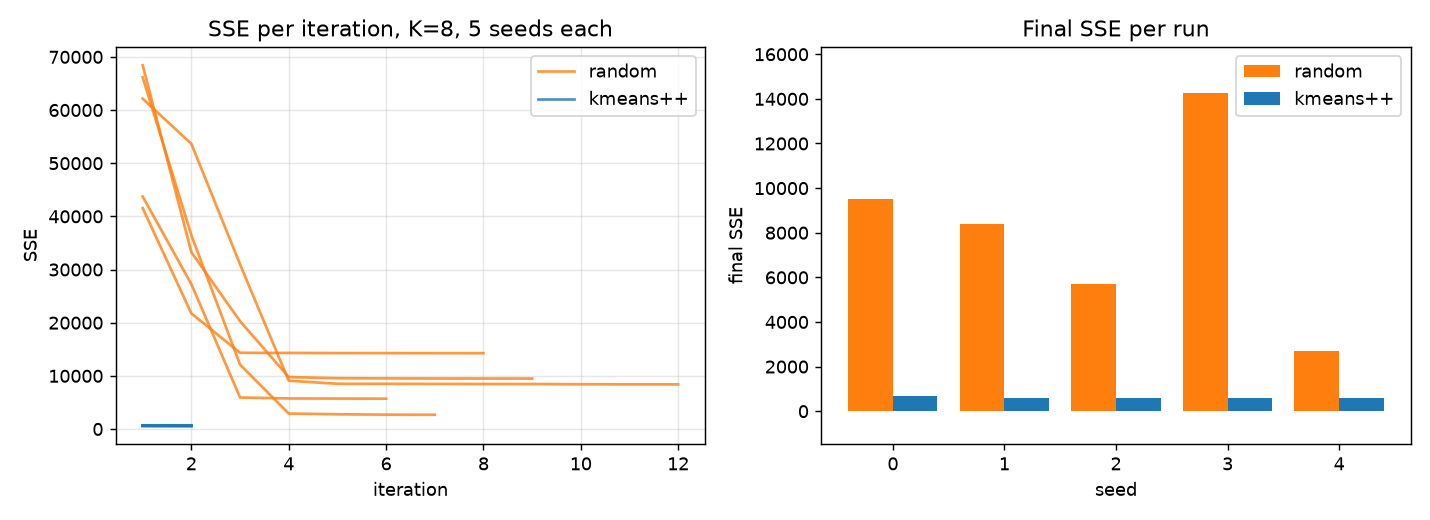
\includegraphics[width=0.92\textwidth]{b_init_comparison.png}
\caption{\texttt{sample2}, $K=8$. Left: SSE per iteration for all 10 runs. Right: final SSE per seed.}
\end{figure}

\textbf{The same experiment on all five images} shows that the advantage is not universal:

\begin{table}[H]\centering\small
\begin{tabular}{lrrrr}
\toprule
image & random: mean SSE (std) & K-Means++: mean SSE (std) & random iters & K-Means++ iters\\
\midrule
sample1 & \textbf{1112} (0.3) & 1171 (75.9) & 42.6 & 32.4\\
sample2 & 8108 (3875) & \textbf{611} (43) & 8.4 & 2.0\\
sample3 & \textbf{317.0} (0.3) & 317.5 (2.7) & 48.6 & 35.8\\
sample4 & 356.8 (29.0) & \textbf{334.2} (26.8) & 45.0 & 39.8\\
sample5 & 1009 (26.4) & \textbf{967.3} (0.0) & 36.2 & 34.8\\
\bottomrule
\end{tabular}
\caption{5 seeds per method, $K=8$. K-Means++ always converges in fewer iterations.}
\end{table}

K-Means++ wins clearly on \texttt{sample2}, \texttt{sample4} and \texttt{sample5}, ties on \texttt{sample3},
and loses on \texttt{sample1}. In \texttt{sample1}, $D^2$ sampling is drawn to rare extreme colours
(white stripes, dark shadows), so it can spend a seed on them while the dominant greens need several.
Random seeds follow the pixel density, which happens to suit that image. Overall, K-Means++ gives lower
or equal SSE on 4 of the 5 images and always needs fewer iterations. Running a few restarts and keeping
the lowest SSE removes the remaining variance with either method.

\subsection{Convergence}

Every image was run with $K=8$ and random initialisation (seed 0), with snapshots after iterations 1, 2 and 5
and at the final iteration. \textbf{The SSE curve never increases on any image} (checked numerically in the code).
This matches the theory. The assignment step gives each pixel its closest centroid, which cannot raise the
SSE. The update step moves each centroid to the mean of its pixels, which is the point minimising their
summed squared distance. Re-seeding an empty cluster does not raise the SSE either, because no pixel
belongs to it.

\begin{table}[H]\centering\small
\begin{tabular}{lrrrc}
\toprule
image & iterations & SSE after iter 1 & final SSE & never increases\\
\midrule
sample1 & 50 & 2072 & 1113 & yes\\
sample2 & 9 & 68430 & 9491 & yes\\
sample3 & 48 & 732.6 & 316.8 & yes\\
sample4 & 50 & 1520 & 372.1 & yes\\
sample5 & 49 & 1218 & 1051 & yes\\
\bottomrule
\end{tabular}
\caption{Convergence with $K=8$ and random initialisation.}
\end{table}

Most of the SSE reduction happens in the first 2--5 iterations. Afterwards, centroids drift slowly between
similar shades (for example the greens in \texttt{sample1}), so the 0.1\% rule is often not met before the 50-iteration cap.
In \texttt{sample1} a second drop appears around iteration 30, when one centroid moves from a crowded green
region to the orange of the fish. The images change visibly only in the first few iterations.

\begin{figure}[H]\centering
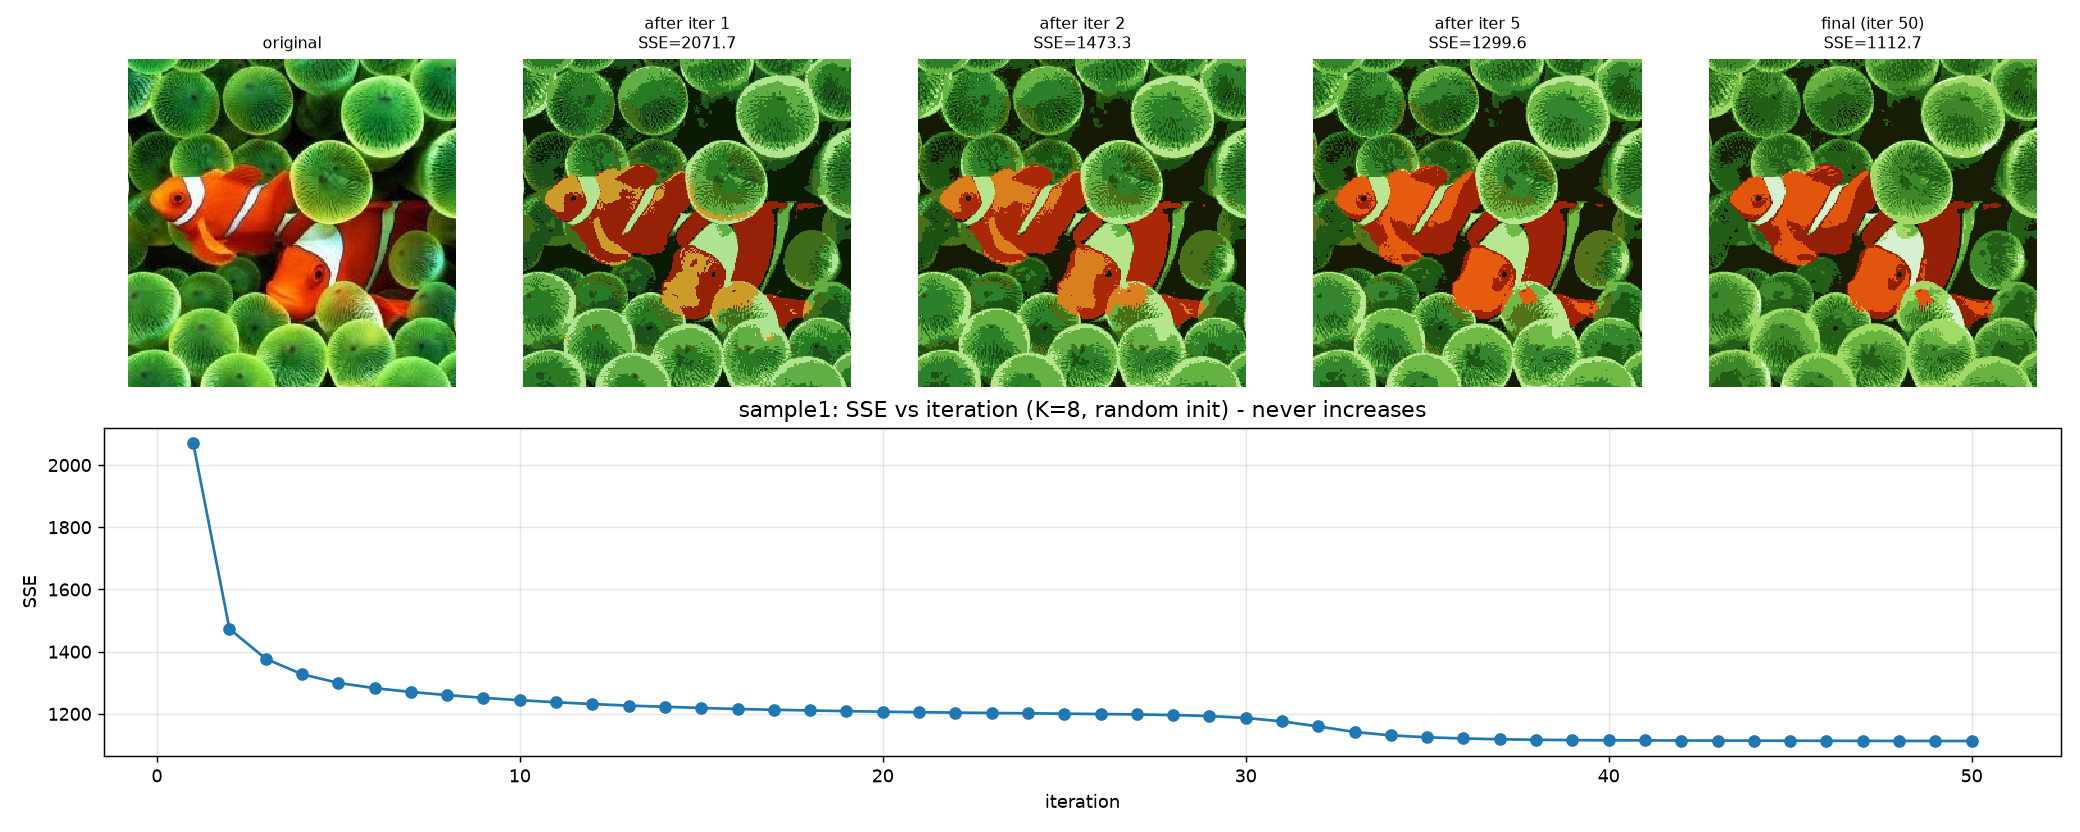
\includegraphics[width=\textwidth]{c_convergence_sample1.png}\\[2pt]
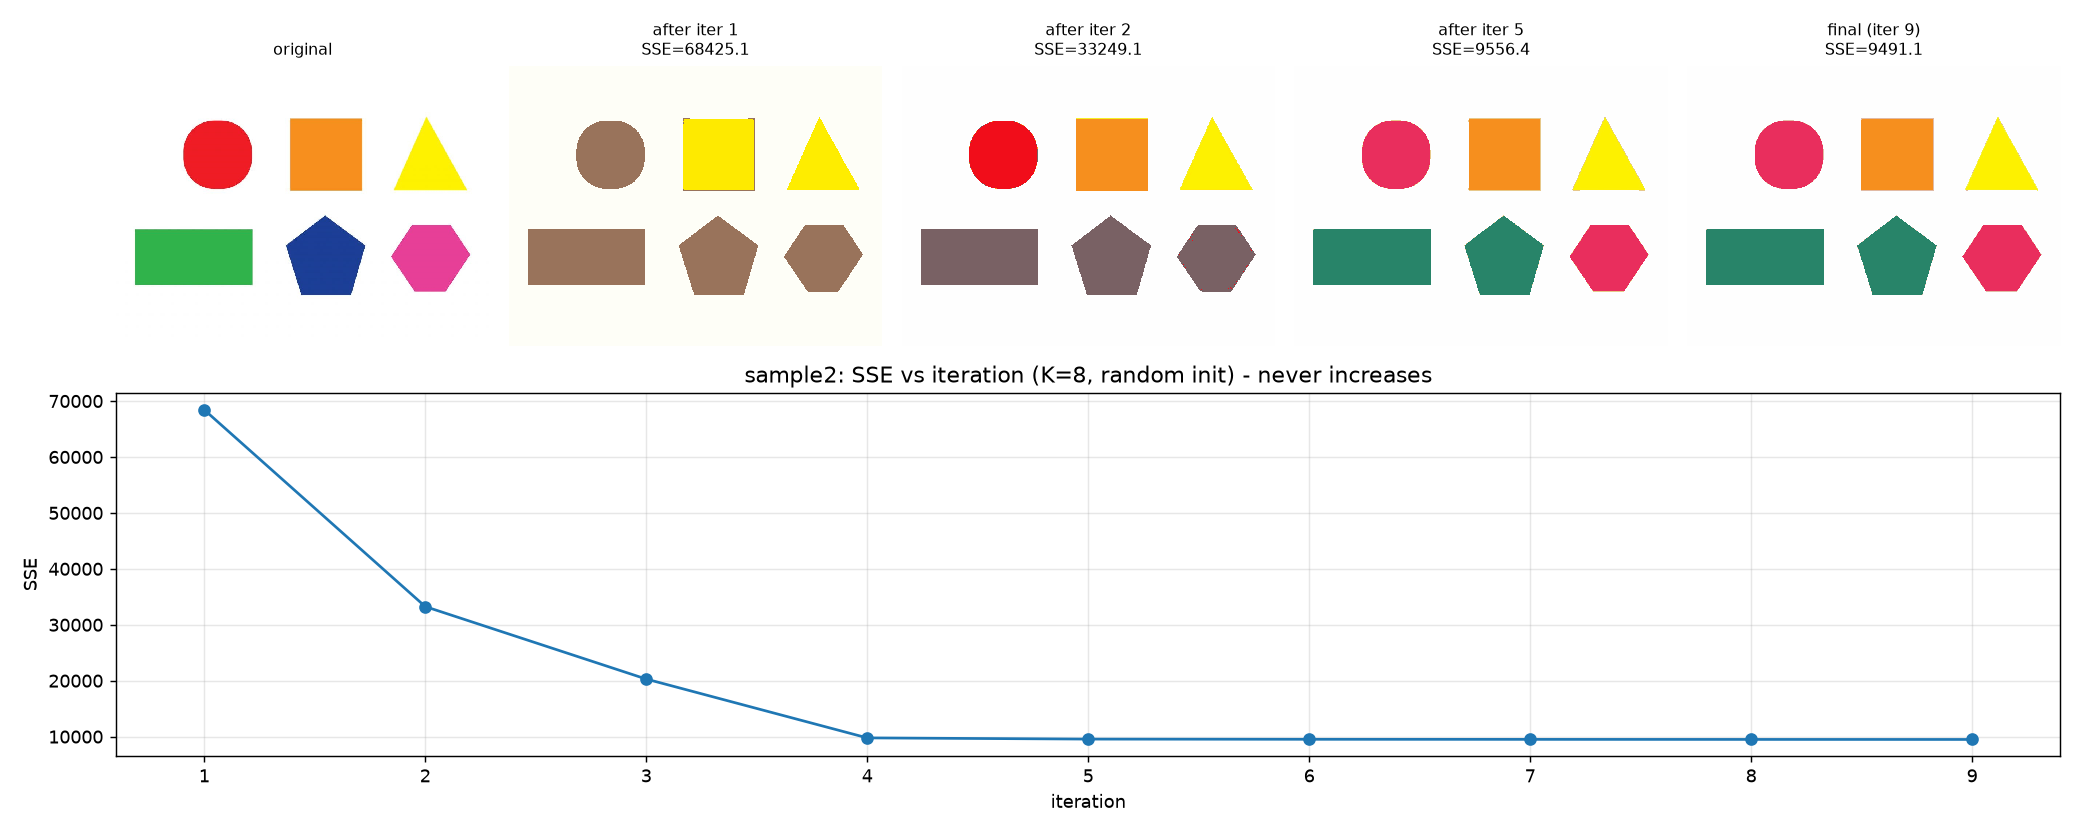
\includegraphics[width=\textwidth]{c_convergence_sample2.png}
\caption{Quantized image after iterations 1, 2, 5 and the final iteration, with the SSE curve
(\texttt{sample1}, \texttt{sample2}).}
\end{figure}
\begin{figure}[H]\centering
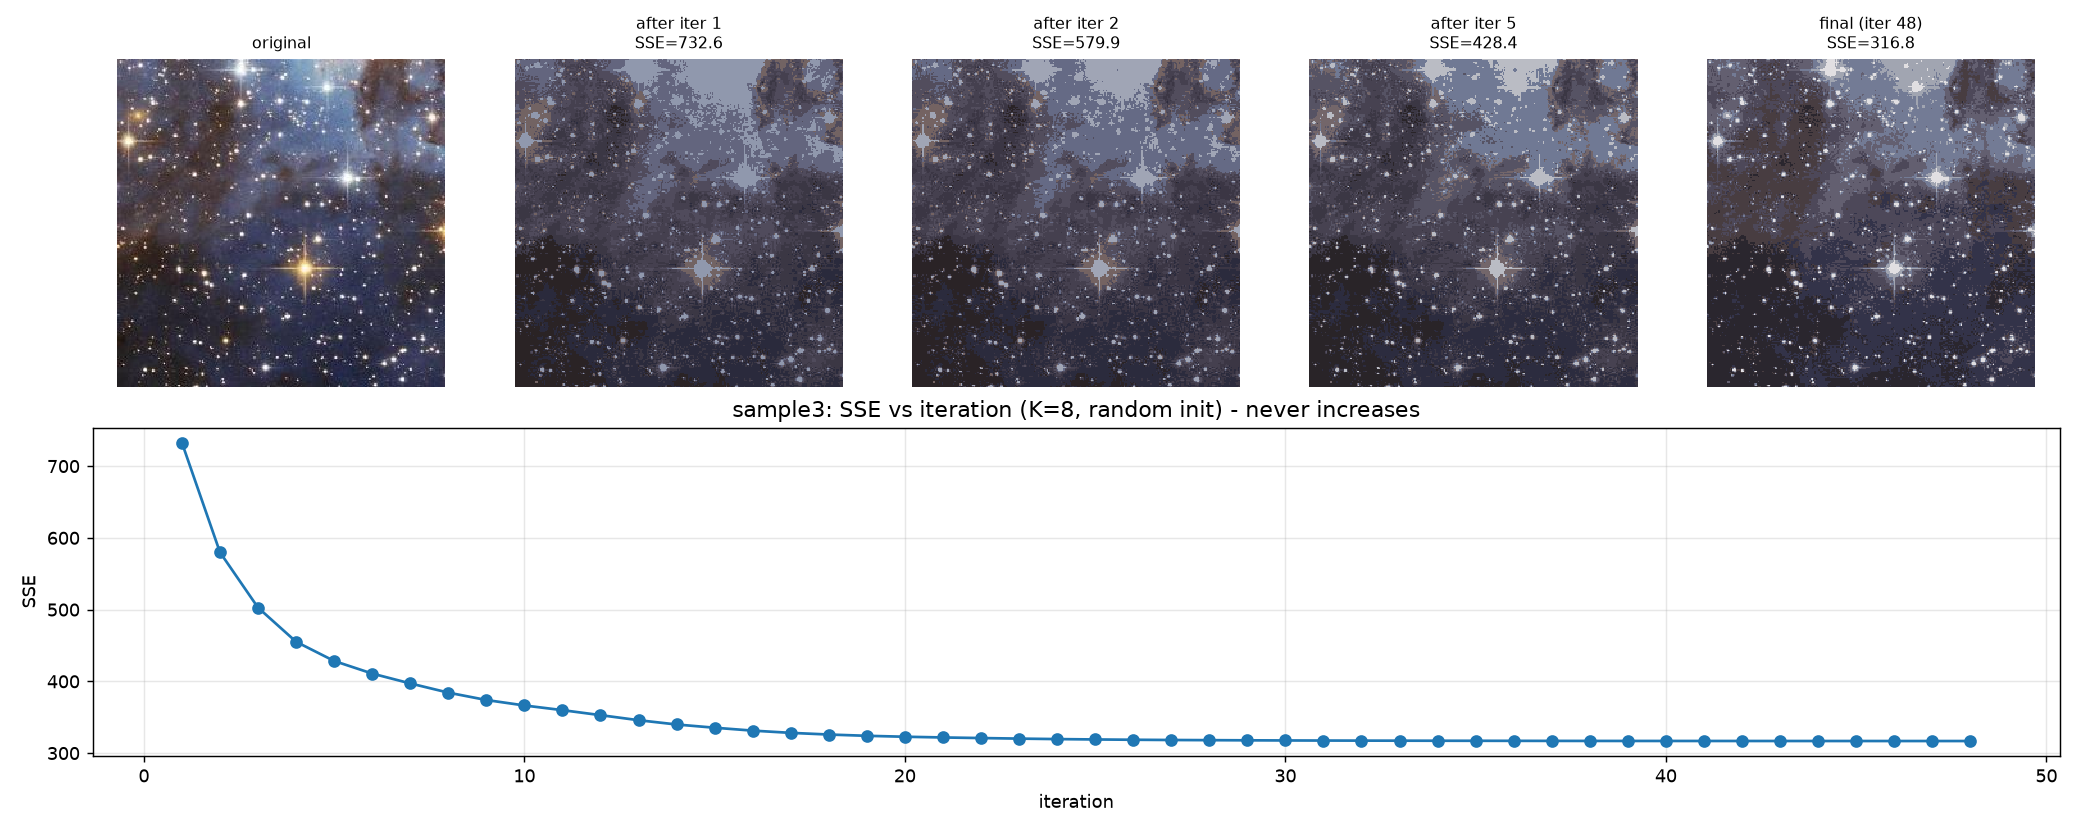
\includegraphics[width=\textwidth]{c_convergence_sample3.png}\\[2pt]
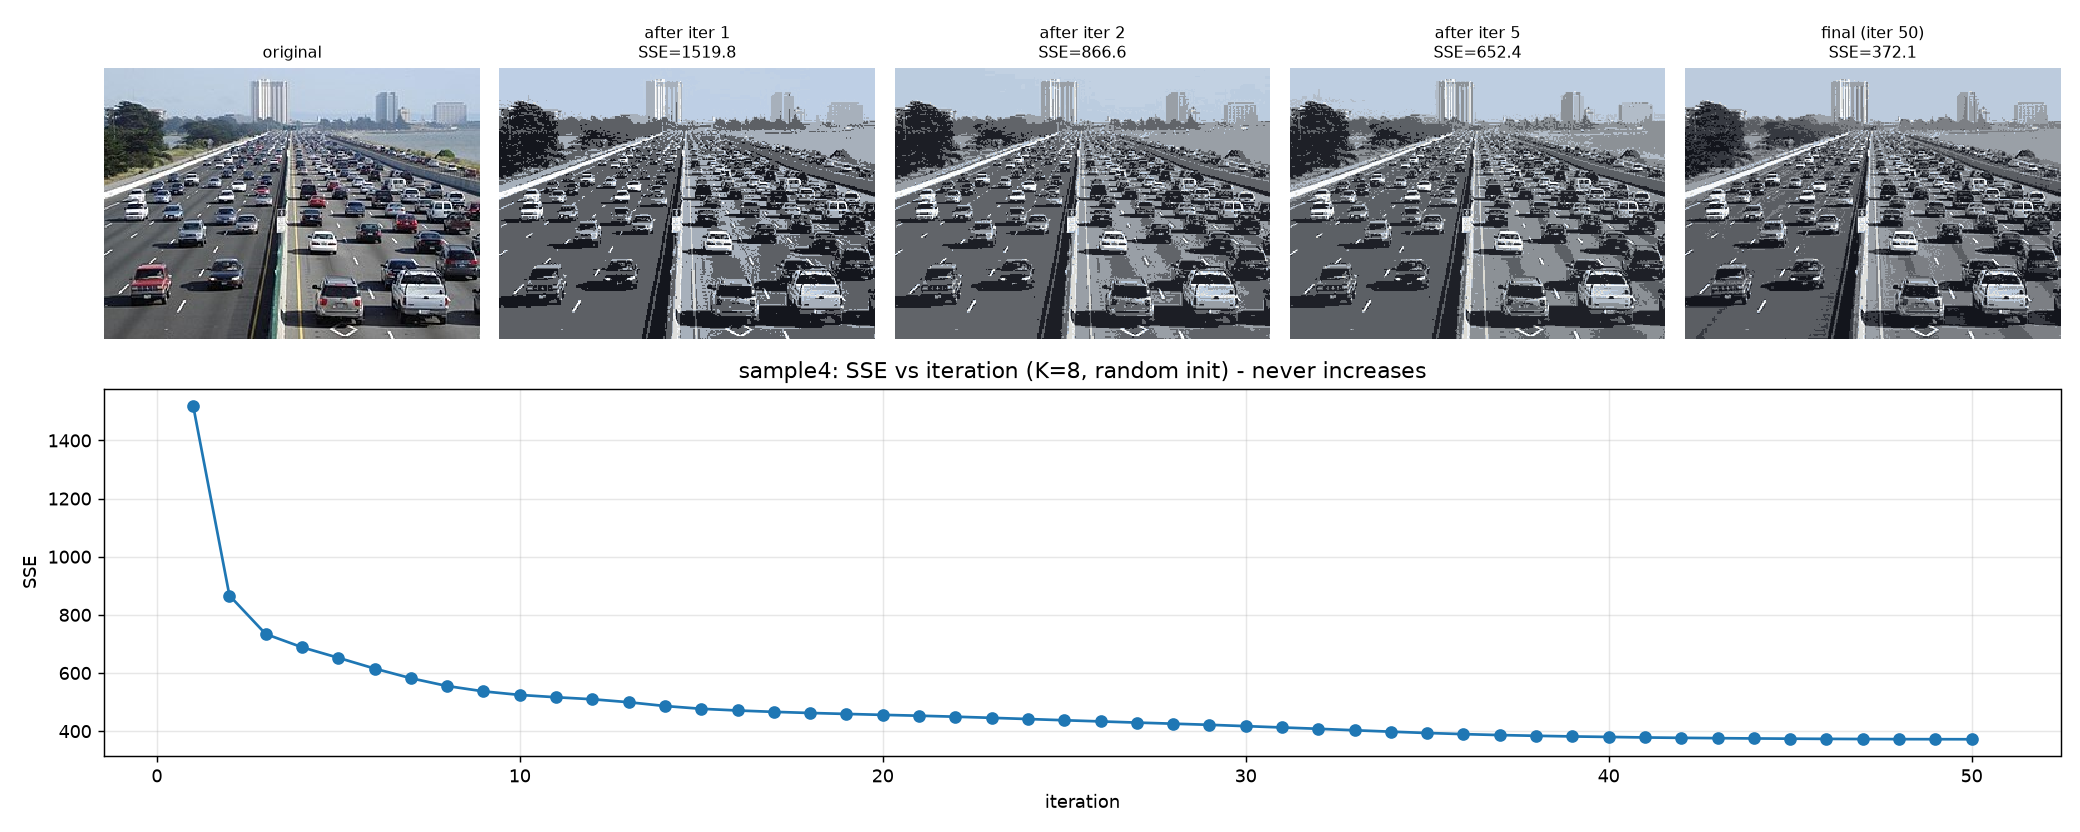
\includegraphics[width=\textwidth]{c_convergence_sample4.png}\\[2pt]
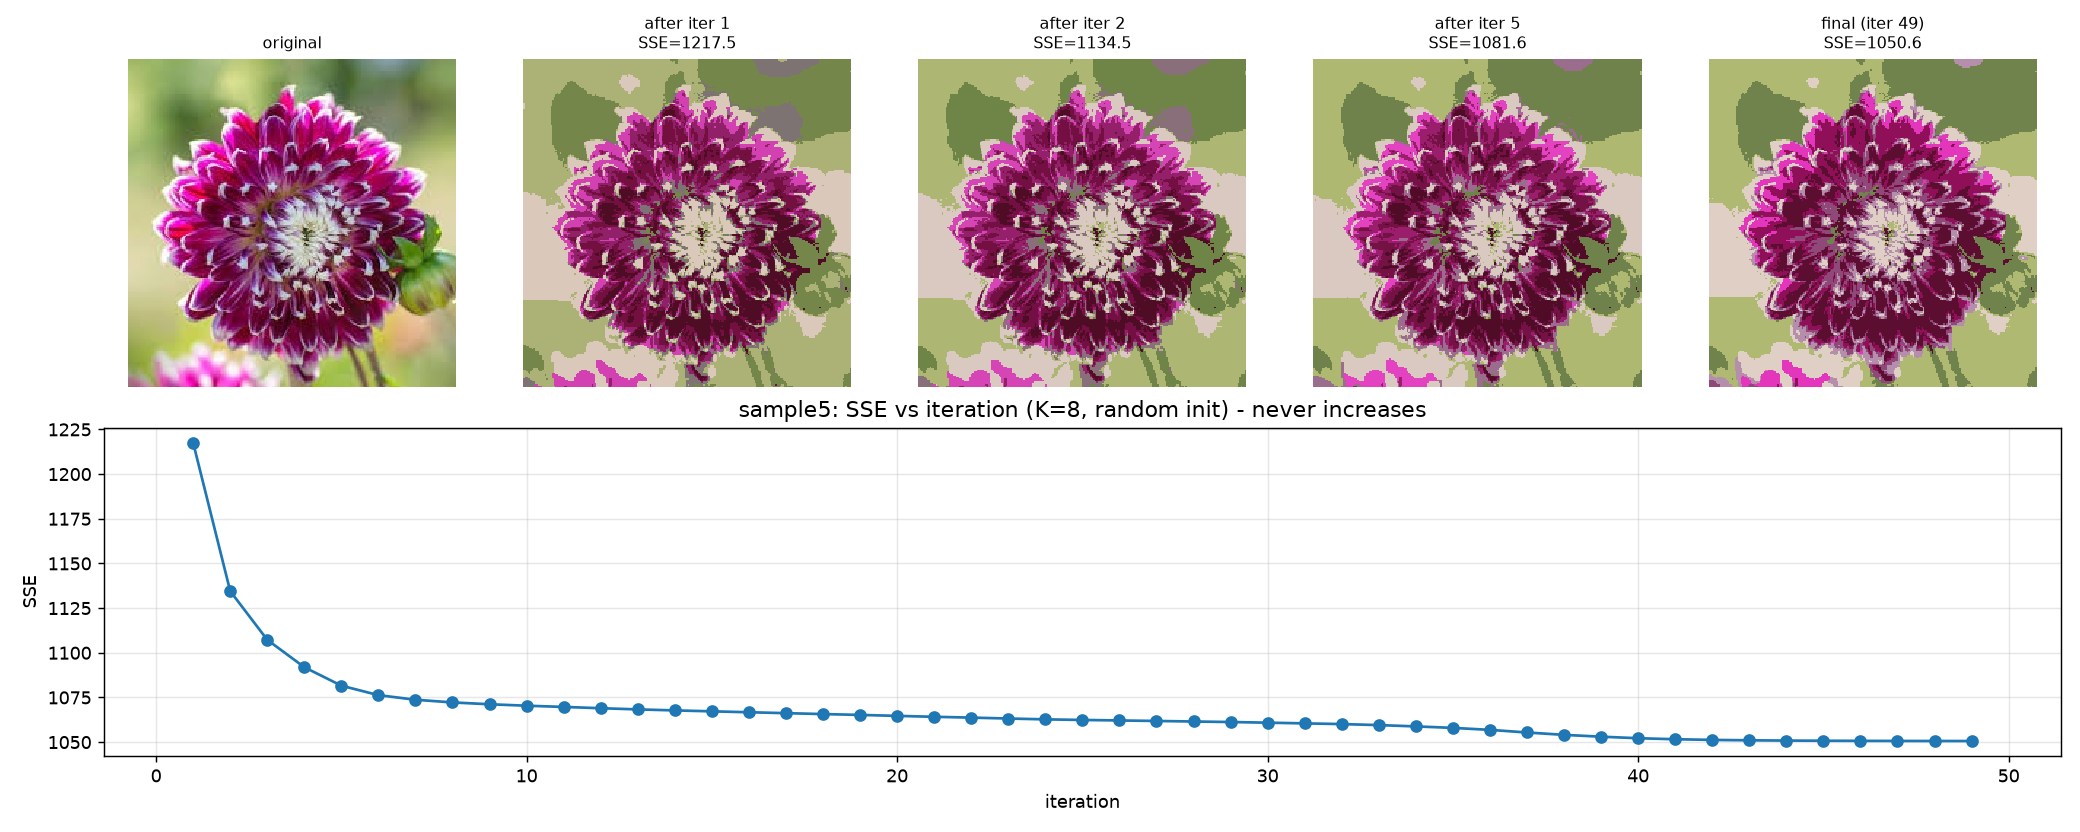
\includegraphics[width=\textwidth]{c_convergence_sample5.png}
\caption{Convergence for \texttt{sample3}, \texttt{sample4}, \texttt{sample5}.}
\end{figure}

\subsection{Choosing $K$}

All runs use K-Means++ (seed 0). The compression ratio is
$\mathrm{CR}(K)=24/(\log_2K+24K/n)$. The palette term $24K/n$ is negligible for these image sizes,
so the CR is almost exactly $24/\log_2K$.

\begin{table}[H]\centering\small
\begin{tabular}{lrrrrr}
\toprule
 & $K=2$ & $K=4$ & $K=8$ & $K=16$ & $K=32$\\
\midrule
SSE sample1 & 6012 & 2473 & 1205 & 621.4 & 375.4\\
SSE sample2 & 53750 & 11960 & 696.9 & 249.9 & 87.3\\
SSE sample3 & 1720 & 662.3 & 316.8 & 161.3 & 85.9\\
SSE sample4 & 3628 & 835.6 & 387.8 & 166.2 & 90.5\\
SSE sample5 & 3860 & 2137 & 967.3 & 517.3 & 309.7\\
\midrule
CR ($256\times256$, $n=65{,}536$) & 23.98 & 11.99 & 7.99 & 5.99 & 4.79\\
CR ($1024\times770$, $n=788{,}480$) & 24.00 & 12.00 & 8.00 & 6.00 & 4.80\\
\bottomrule
\end{tabular}
\caption{Final SSE and compression ratio for each $K$.
(\texttt{sample4}/\texttt{sample5} CRs differ from the $256\times256$ row by at most 0.01.)}
\end{table}

\textbf{Recommendation: $K=16$.} In the elbow plots (log scale on $K$), the absolute SSE gain from each
doubling shrinks quickly. For \texttt{sample1}, the gains are 3539, 1268, 584 and 246, so the curve
flattens between $K=8$ and $K=16$. Visually, $K=8$ still shows banding on smooth gradients (the orange
of the fish, the shading of the anemones, the sky in \texttt{sample4}, the petals in \texttt{sample5}),
while $K=16$ is hard to tell from the original at normal size, and $K=32$ adds little. $K=16$ still
compresses $6\times$ (4 bits per pixel instead of 24). One image-specific exception: \texttt{sample2}
contains only 7 colours plus anti-aliasing, so its elbow is sharply at $K=8$ (SSE falls by 94\% from
$K=4$ to $K=8$), and $K=8$ gives $8\times$ compression with no visible loss there.

\begin{figure}[H]\centering
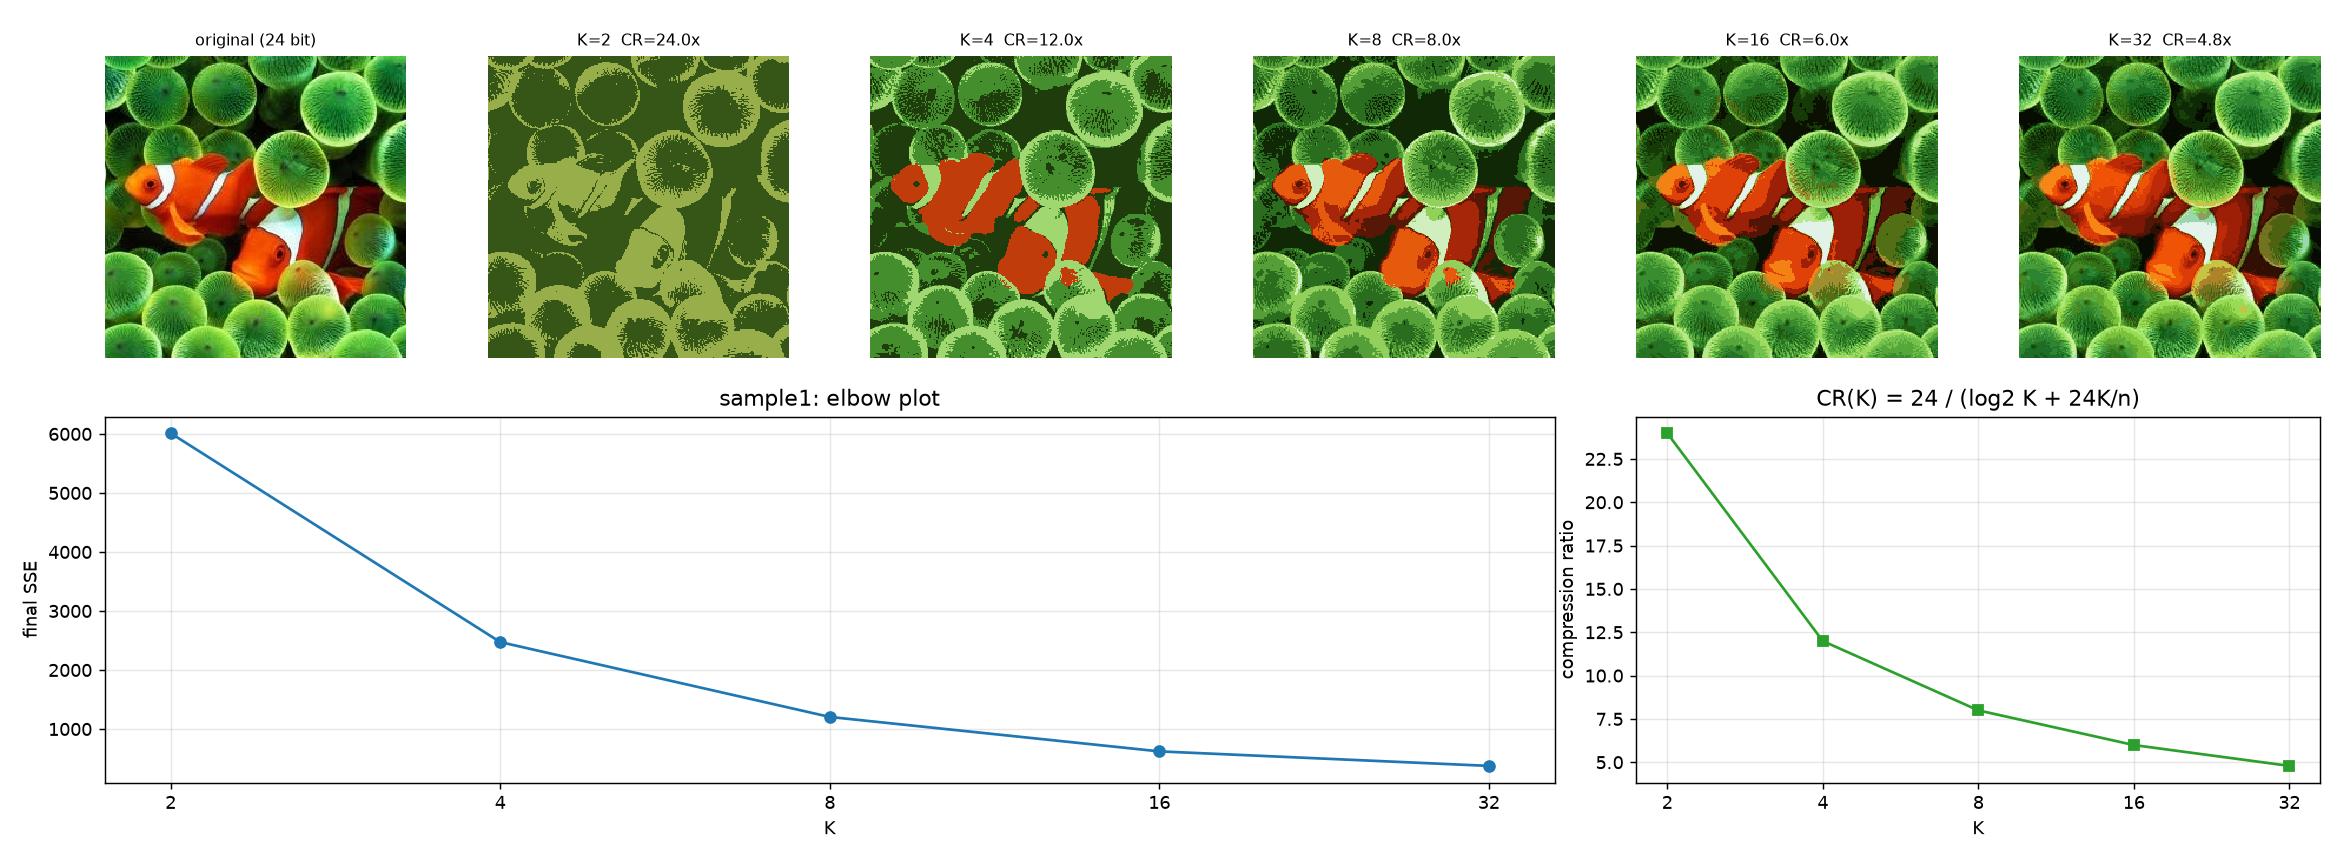
\includegraphics[width=\textwidth]{d_choose_k_sample1.png}\\[2pt]
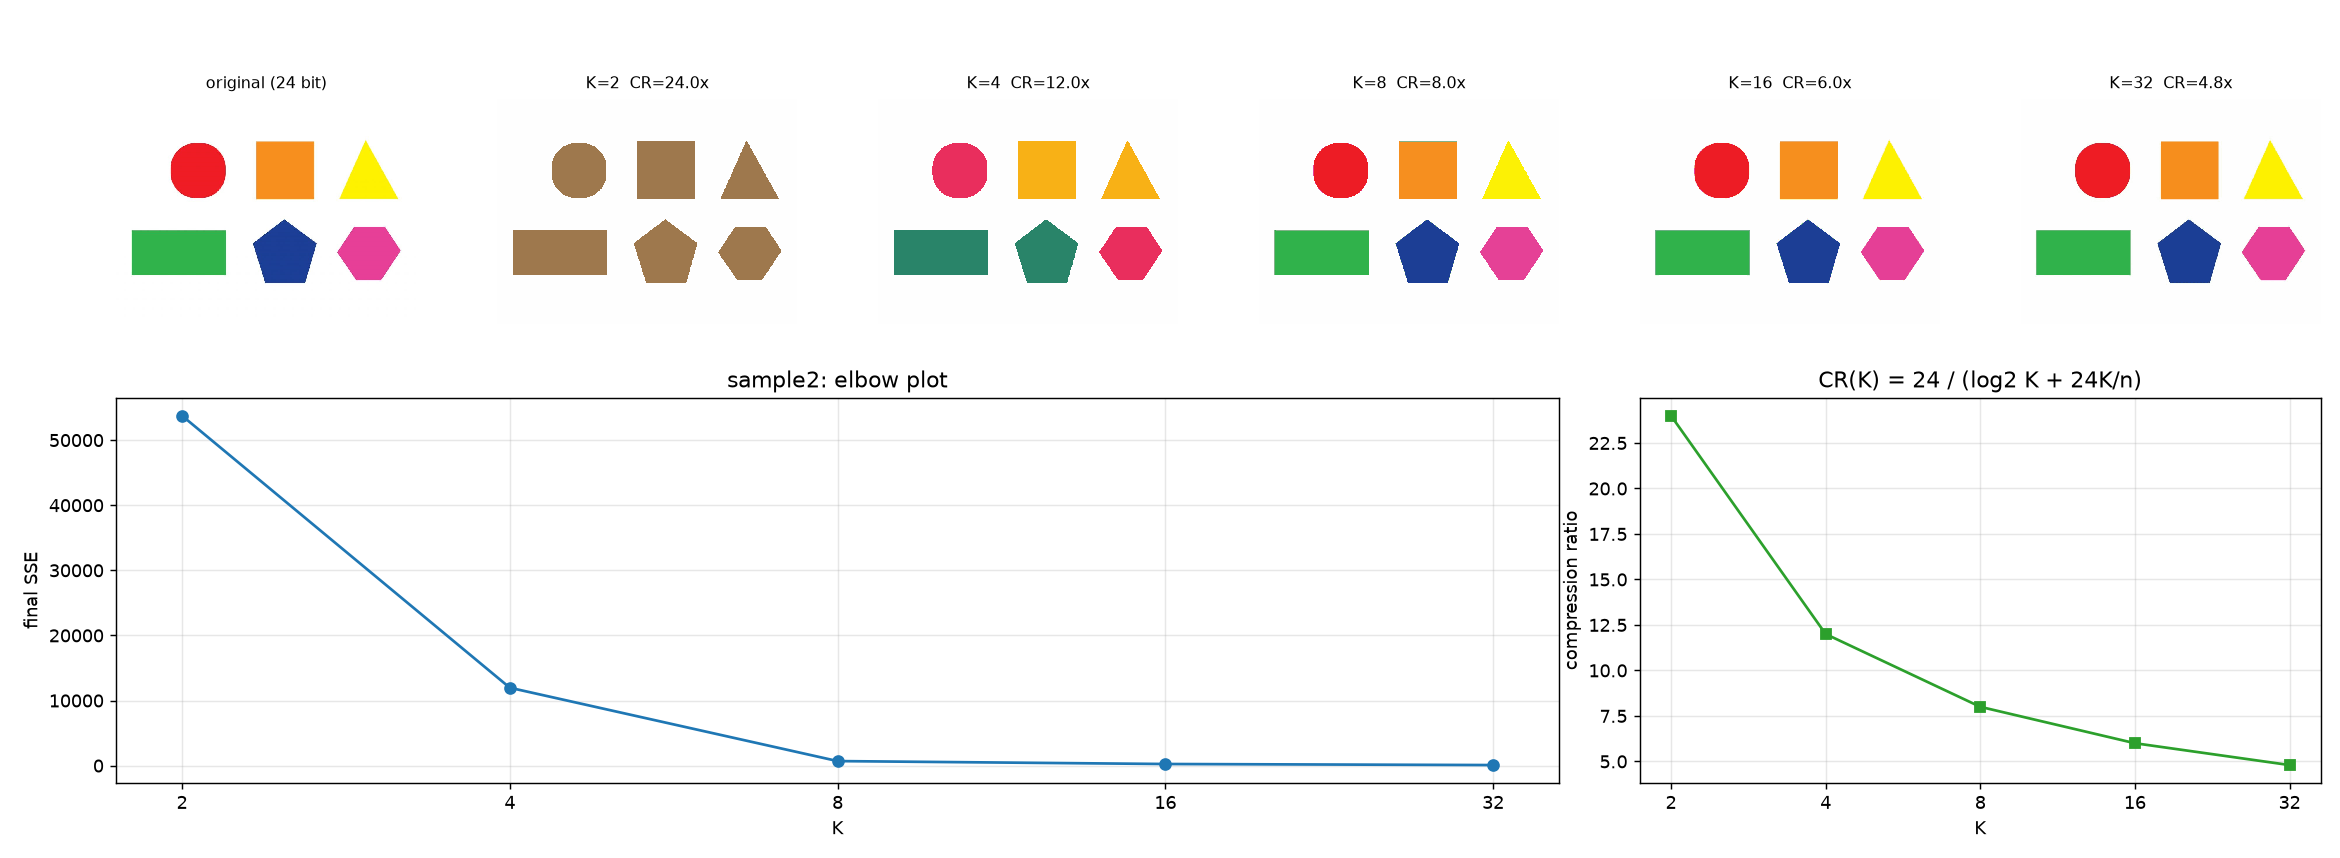
\includegraphics[width=\textwidth]{d_choose_k_sample2.png}
\caption{Quantized images for $K\in\{2,4,8,16,32\}$, elbow plot and compression ratio (\texttt{sample1}, \texttt{sample2}).}
\end{figure}
\begin{figure}[H]\centering
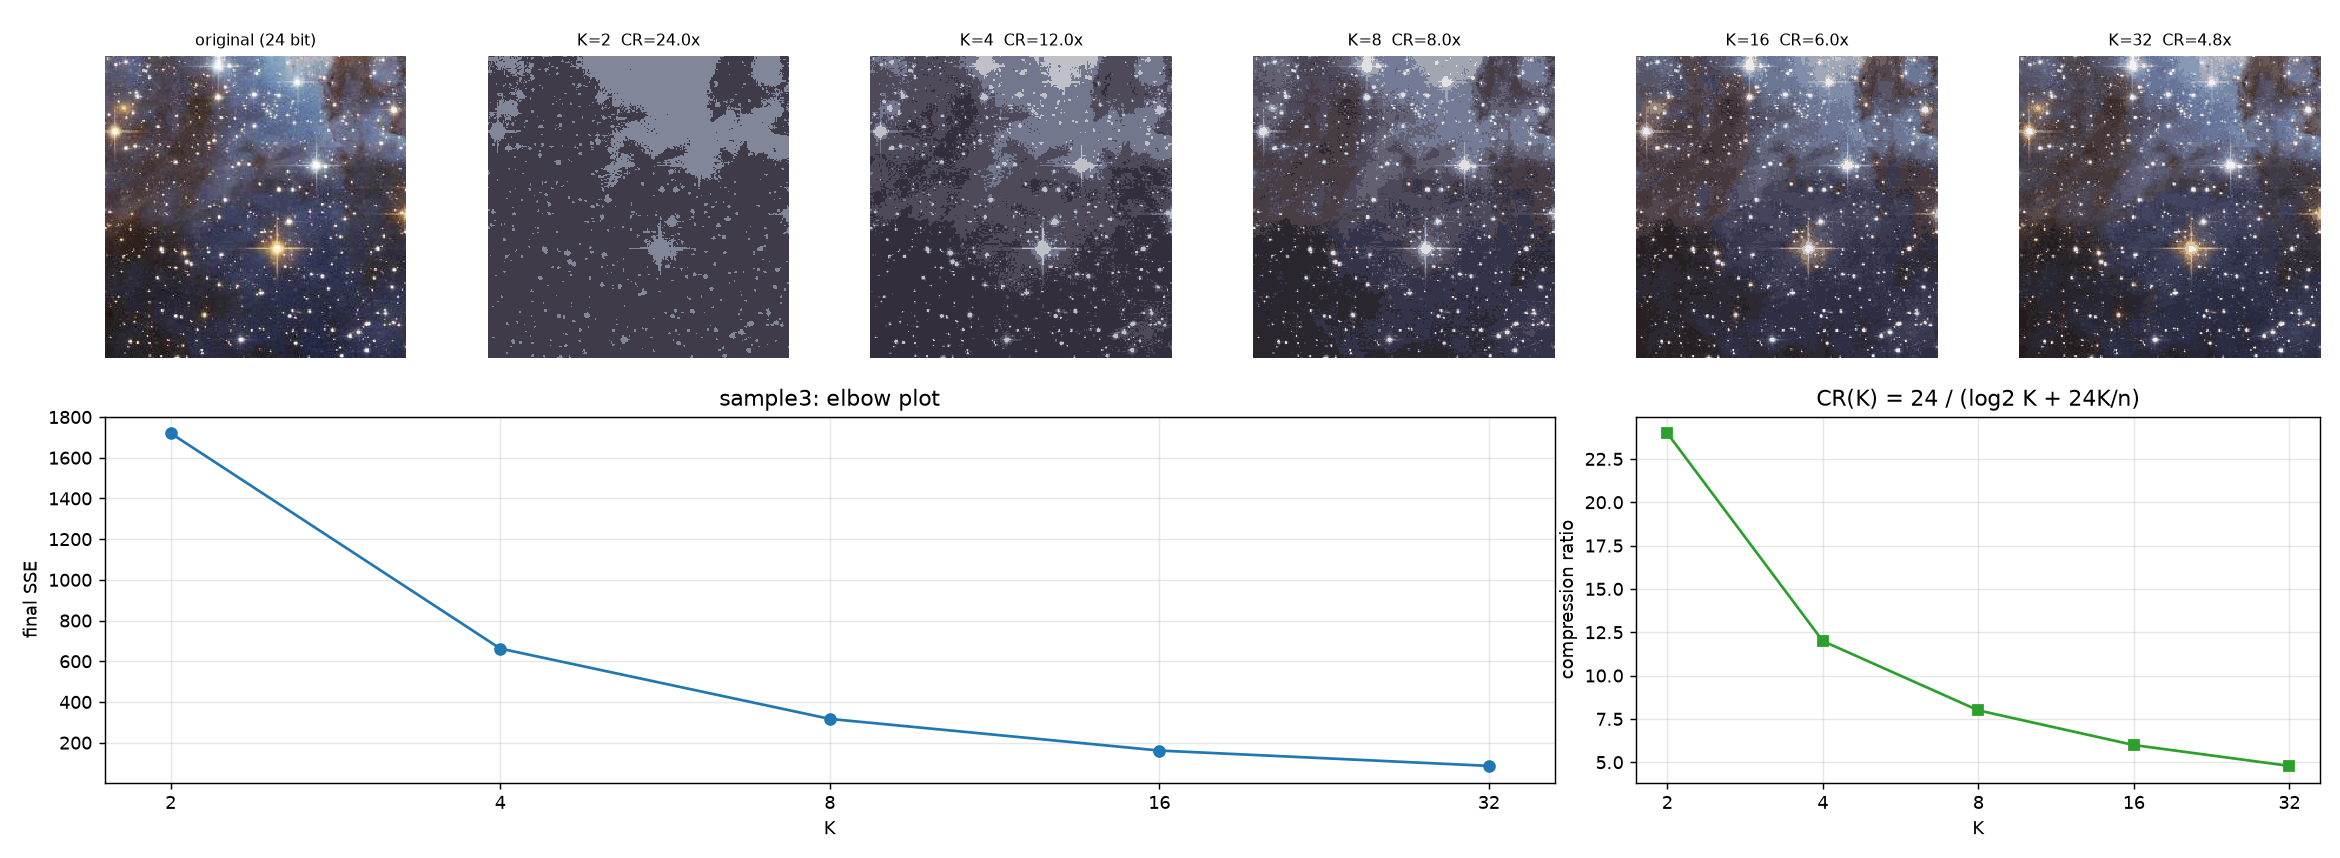
\includegraphics[width=\textwidth]{d_choose_k_sample3.png}\\[2pt]
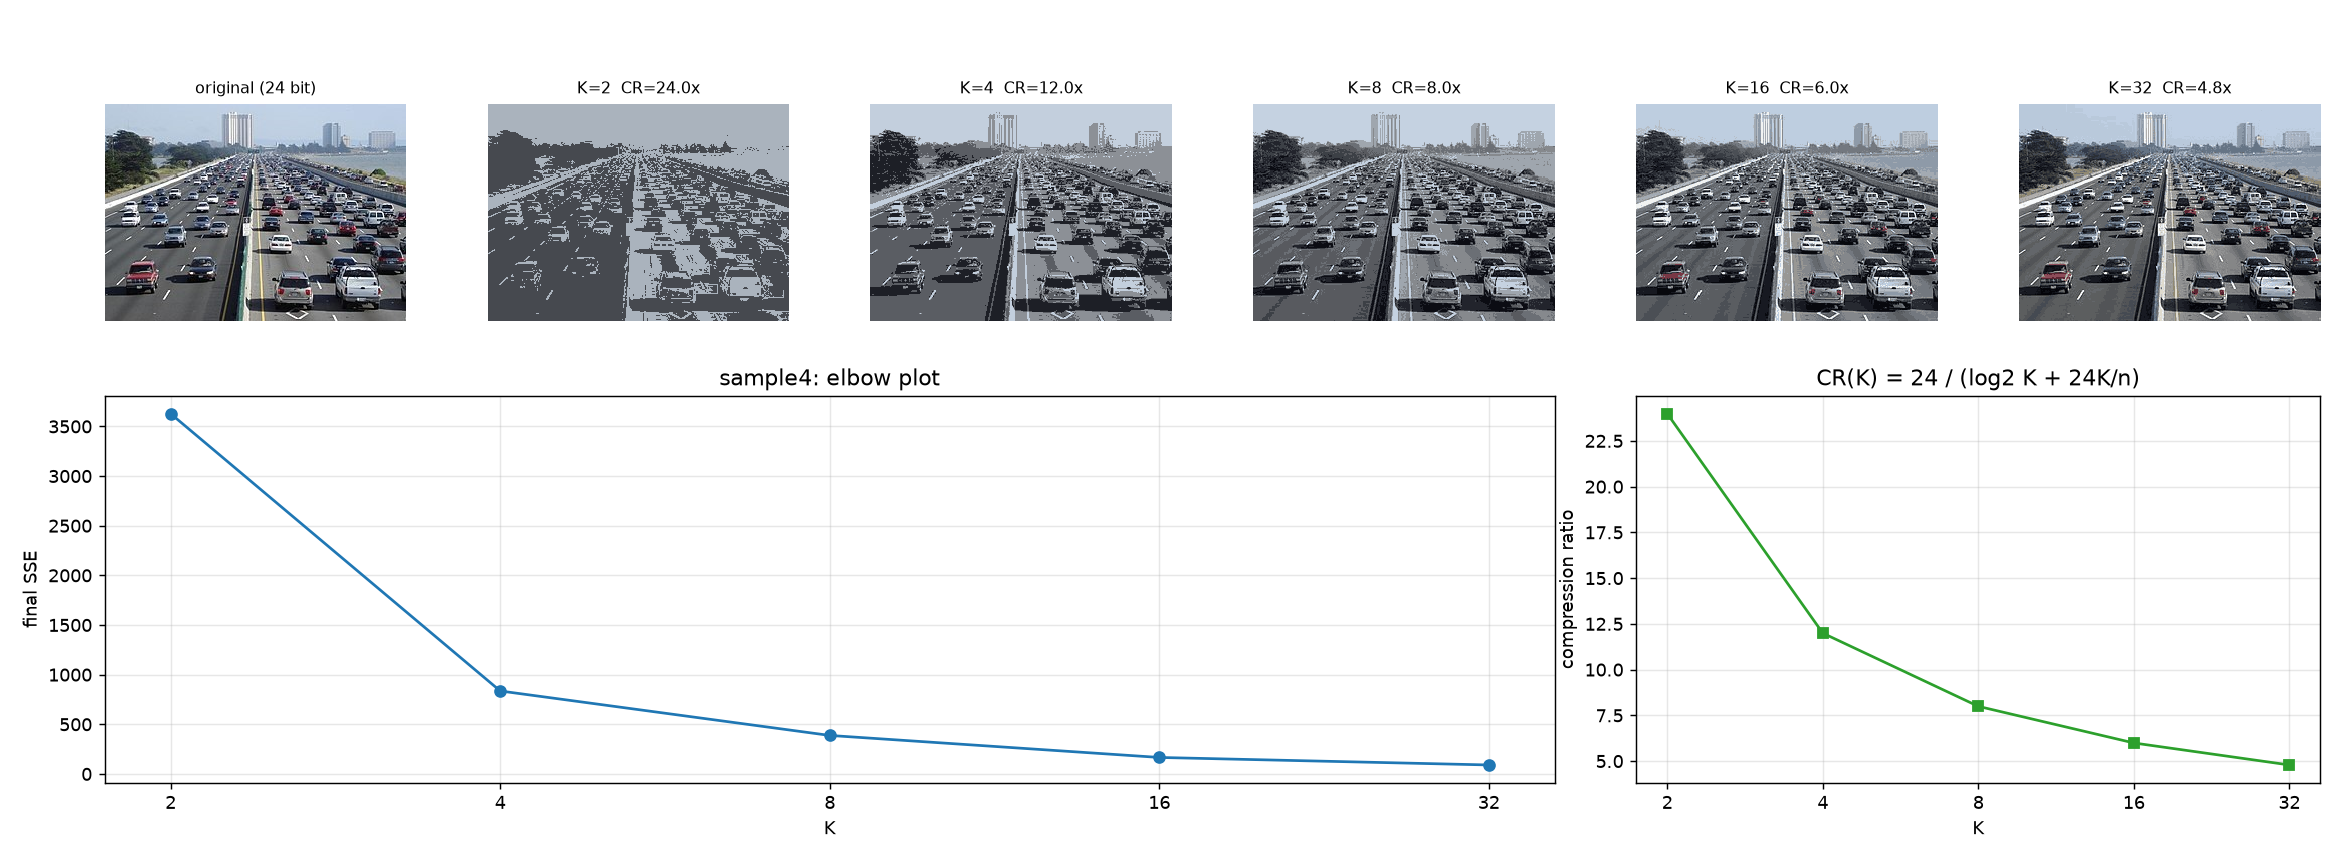
\includegraphics[width=\textwidth]{d_choose_k_sample4.png}\\[2pt]
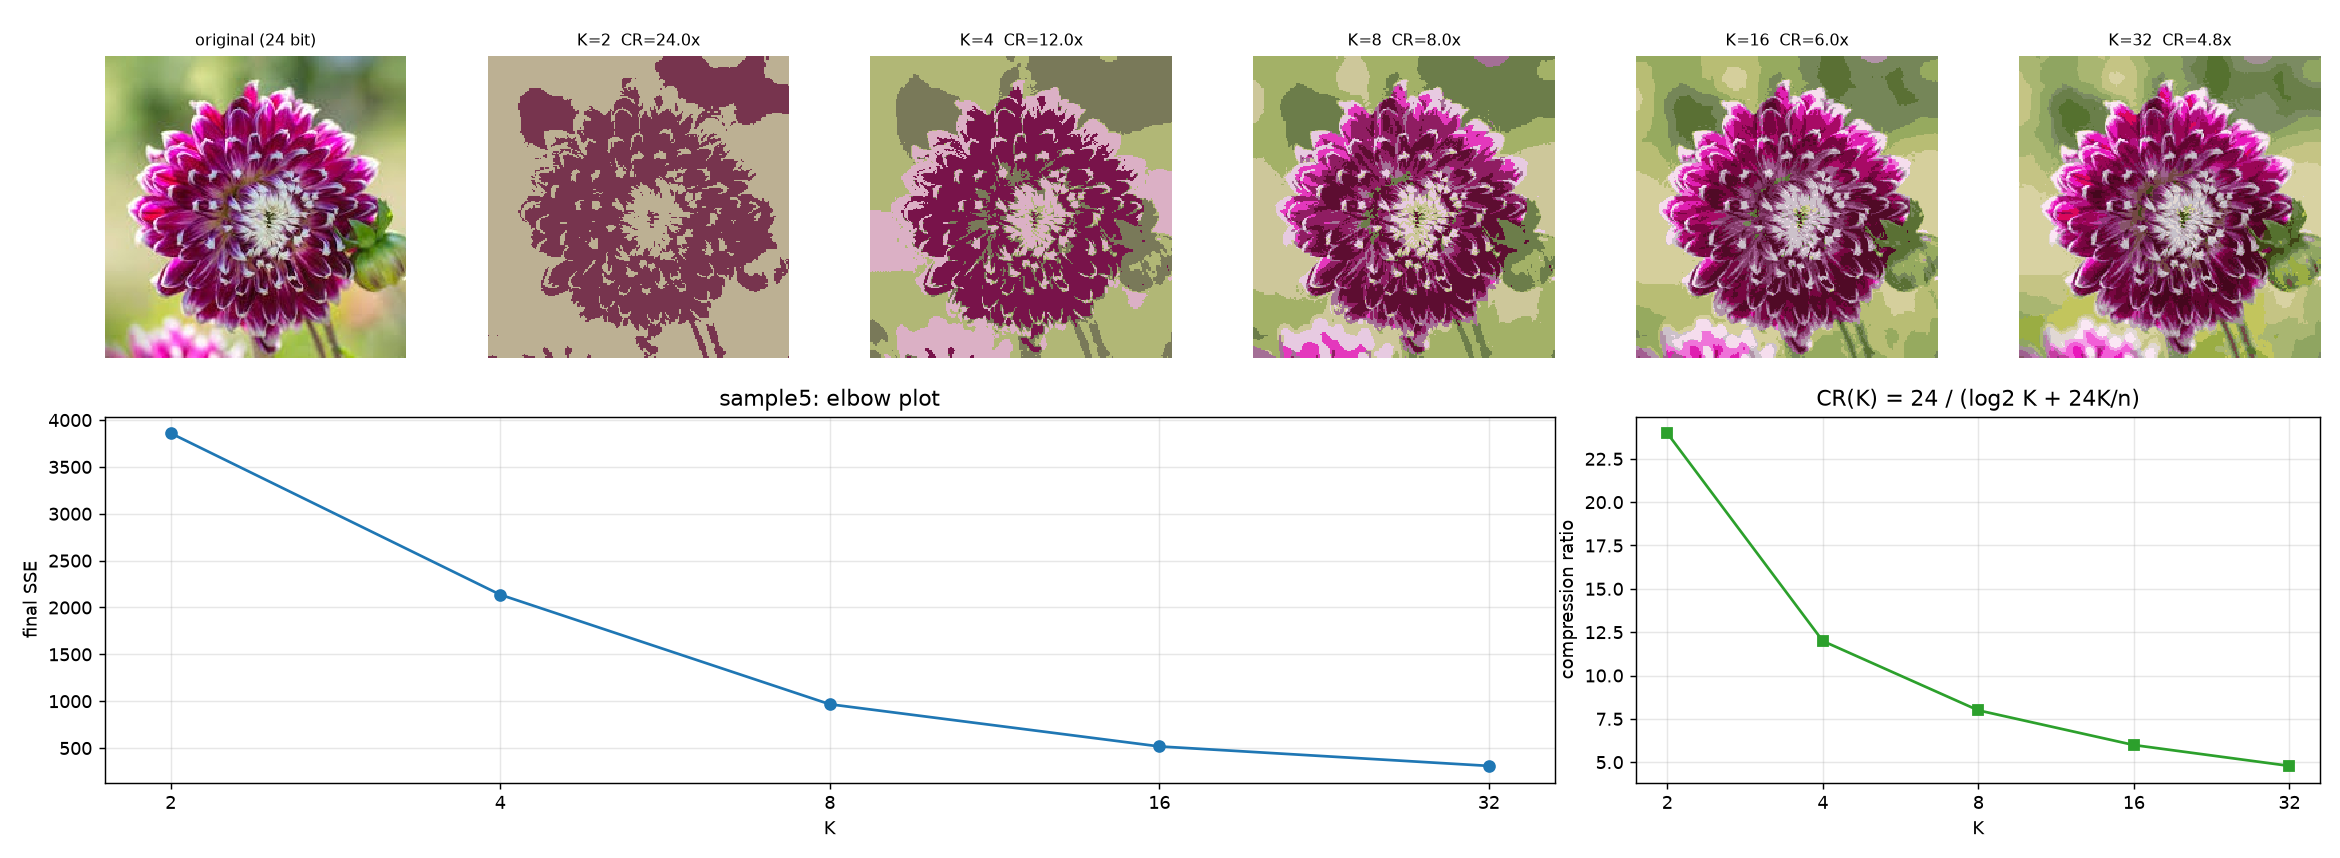
\includegraphics[width=\textwidth]{d_choose_k_sample5.png}
\caption{Choosing $K$ for \texttt{sample3}, \texttt{sample4}, \texttt{sample5}.}
\end{figure}

\subsection{DBSCAN from scratch}

\begin{itemize}
  \item \textbf{Downsampling.} Block averaging with integer factor $f=\lceil\max(H,W)/80\rceil$, giving
        $64\times64$, $78\times59$, $64\times64$, $75\times54$ and $75\times75$ pixels (at most $5{,}625$ points).
  \item \textbf{Neighbourhoods.} \texttt{\_neighbours} computes distances from 1024 points at a time to all points
        and keeps the indices with distance $\le\varepsilon$. A point counts as its own neighbour.
  \item \textbf{Labels.} A point with at least \texttt{minPts} neighbours is \emph{core}.
        Clusters grow from each unvisited core point with a stack, and only core points expand further.
        Non-core points reached this way are \emph{border} points. Everything never reached is \emph{noise}.
  \item \textbf{Choosing $\varepsilon$.} With $\texttt{minPts}=6$ ($=2\times$ the 3 RGB dimensions), we sort every
        point's distance to its 6th nearest neighbour (itself included, so it matches the core test). We take the
        elbow as the point lying farthest below the straight line from the first to the last point of the
        normalised curve.
\end{itemize}

\begin{table}[H]\centering\small
\begin{tabular}{lcrrrrrrrr}
\toprule
image & size & $\varepsilon$ & clusters & clusters $\ge$1\% & core & border & noise & noise \% & time (s)\\
\midrule
sample1 & $64\times64$ & 0.0490 & 5 & 1 & 3658 & 138 & 300 & 7.3 & 0.23\\
sample2 & $78\times59$ & 0.0032 & 20 & 7 & 4345 & 14 & 243 & 5.3 & 0.48\\
sample3 & $64\times64$ & 0.0263 & 7 & 1 & 3888 & 90 & 118 & 2.9 & 0.29\\
sample4 & $75\times54$ & 0.0256 & 4 & 1 & 3750 & 118 & 182 & 4.5 & 0.25\\
sample5 & $75\times75$ & 0.0478 & 10 & 1 & 5128 & 300 & 197 & 3.5 & 0.66\\
\bottomrule
\end{tabular}
\caption{DBSCAN on RGB features with $\varepsilon$ from the k-distance elbow ($\texttt{minPts}=6$).}
\end{table}

\textbf{Observations.} On \texttt{sample2}, DBSCAN finds exactly the 7 real regions (white background and
6 shapes) as its large clusters. The other 13 clusters are tiny strips of anti-aliased edge colour, and
the noise pixels are the blended outlines. On the four natural photographs, DBSCAN returns \textbf{one giant
cluster with 90--95\% of the pixels}, plus a few tiny ones. Their colour distributions are continuous: every
shade has many near-identical neighbours, so density-reachability chains link dark green to light green
(and even to orange through intermediate shades). DBSCAN therefore cannot produce a colour palette for
such images. What it finds instead are the \emph{rare} colours (highlights, the white stripes of the fish,
bright stars), which it marks as noise.

\begin{figure}[H]\centering
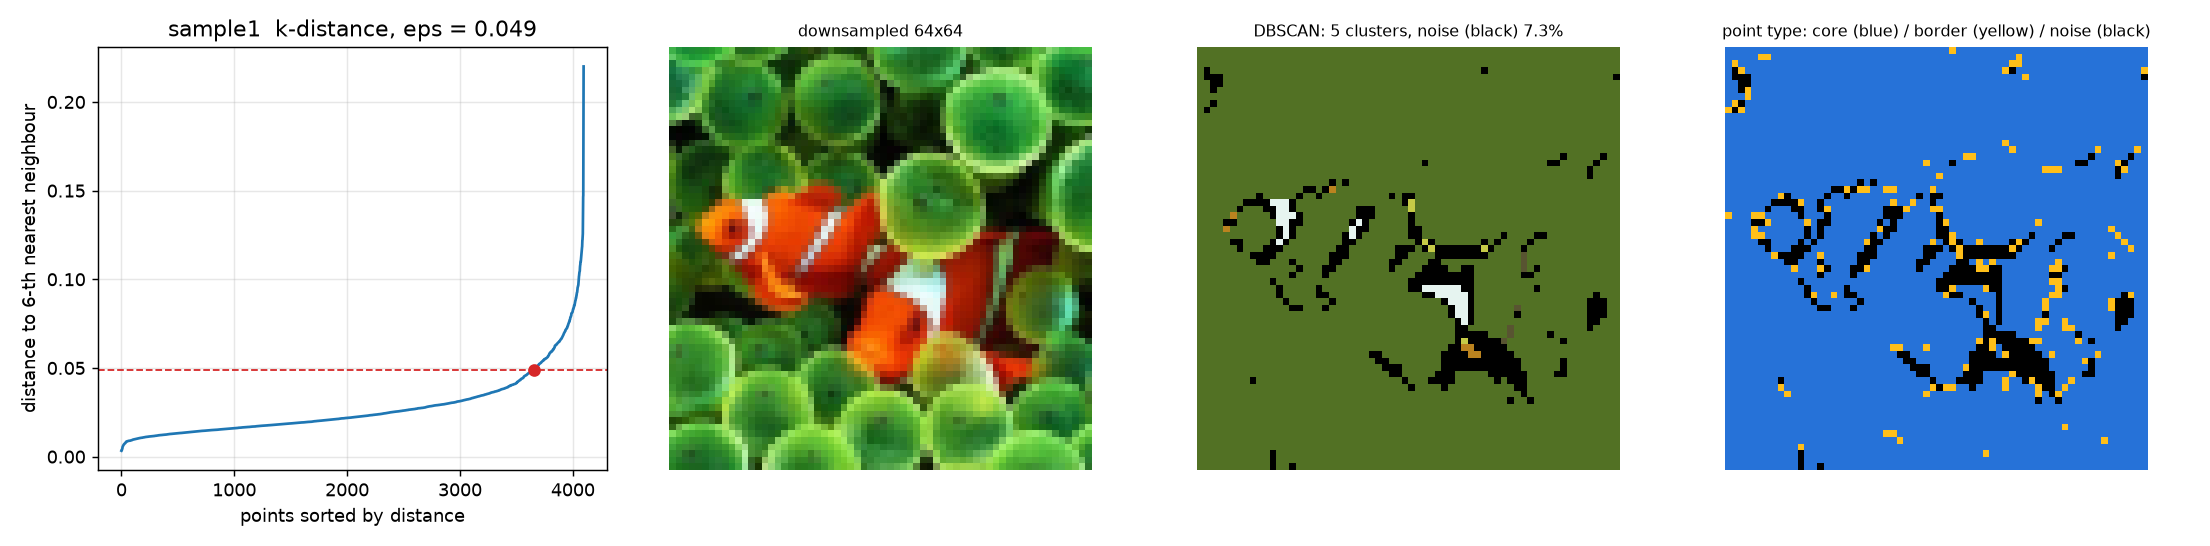
\includegraphics[width=\textwidth]{e_dbscan_sample1.png}\\[2pt]
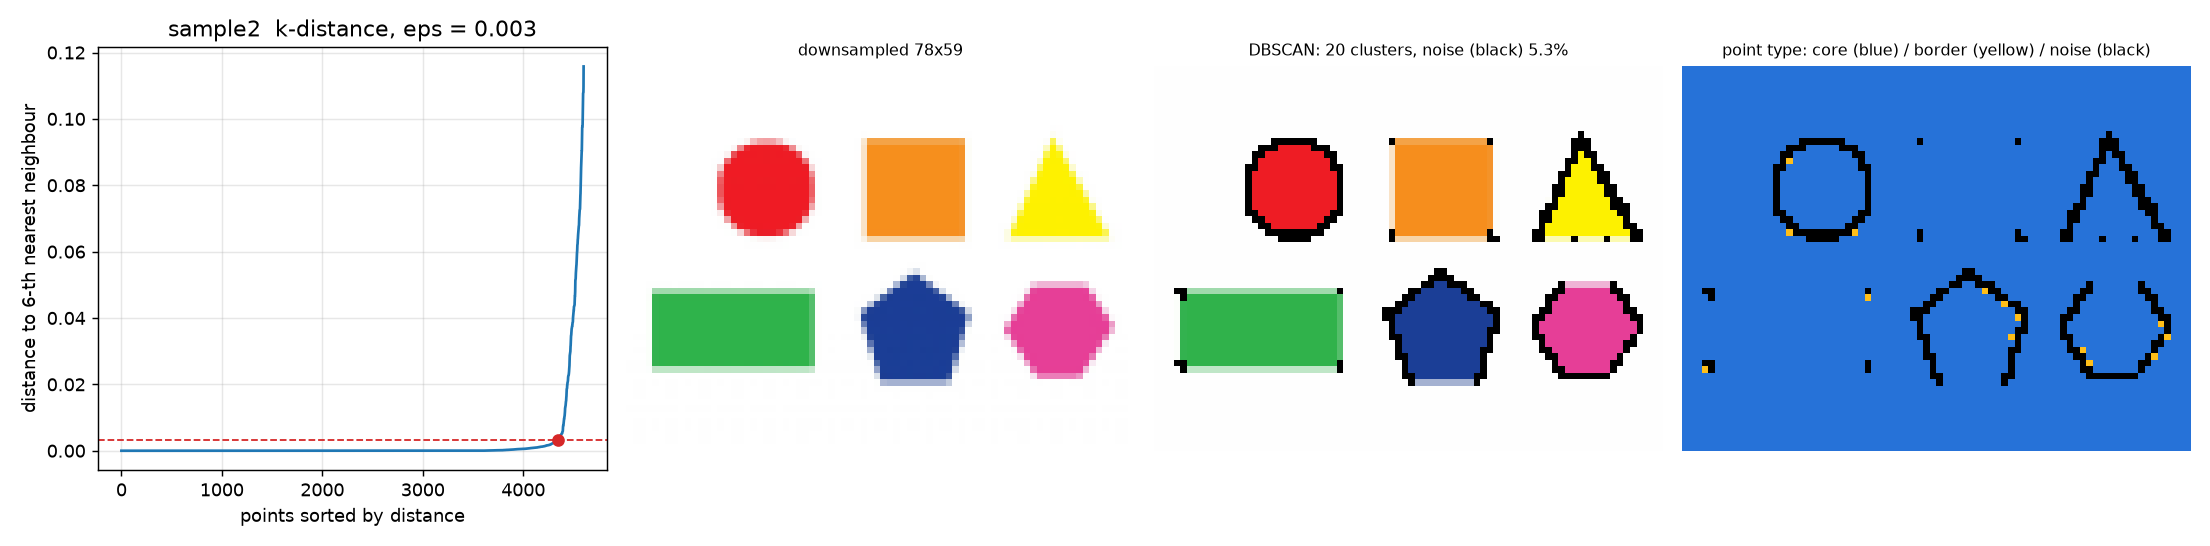
\includegraphics[width=\textwidth]{e_dbscan_sample2.png}\\[2pt]
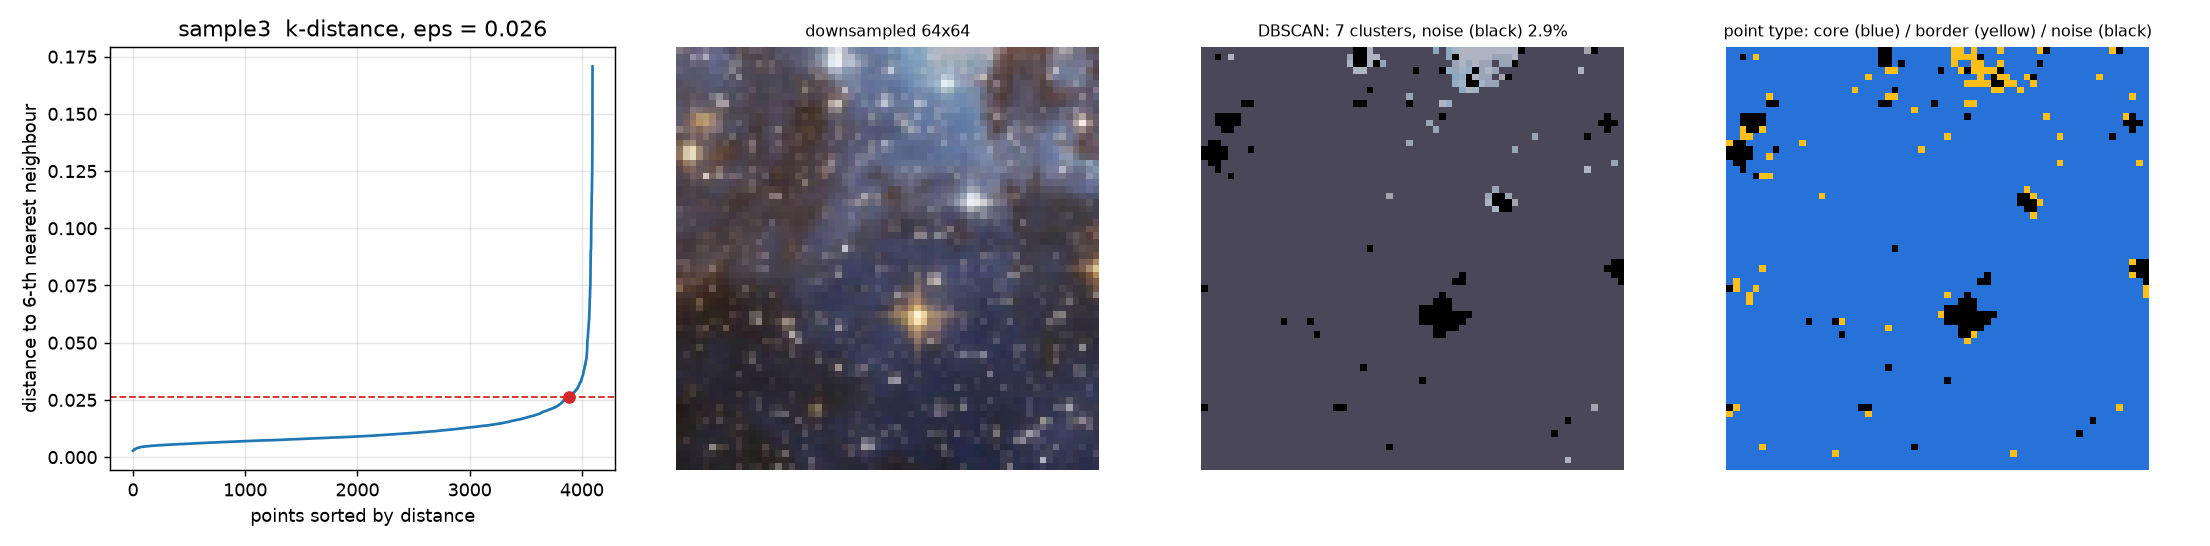
\includegraphics[width=\textwidth]{e_dbscan_sample3.png}
\caption{k-distance plot with the chosen $\varepsilon$, downsampled image, DBSCAN result (each cluster in its mean
colour, noise in black) and point types (\texttt{sample1}--\texttt{sample3}).}
\end{figure}
\begin{figure}[H]\centering
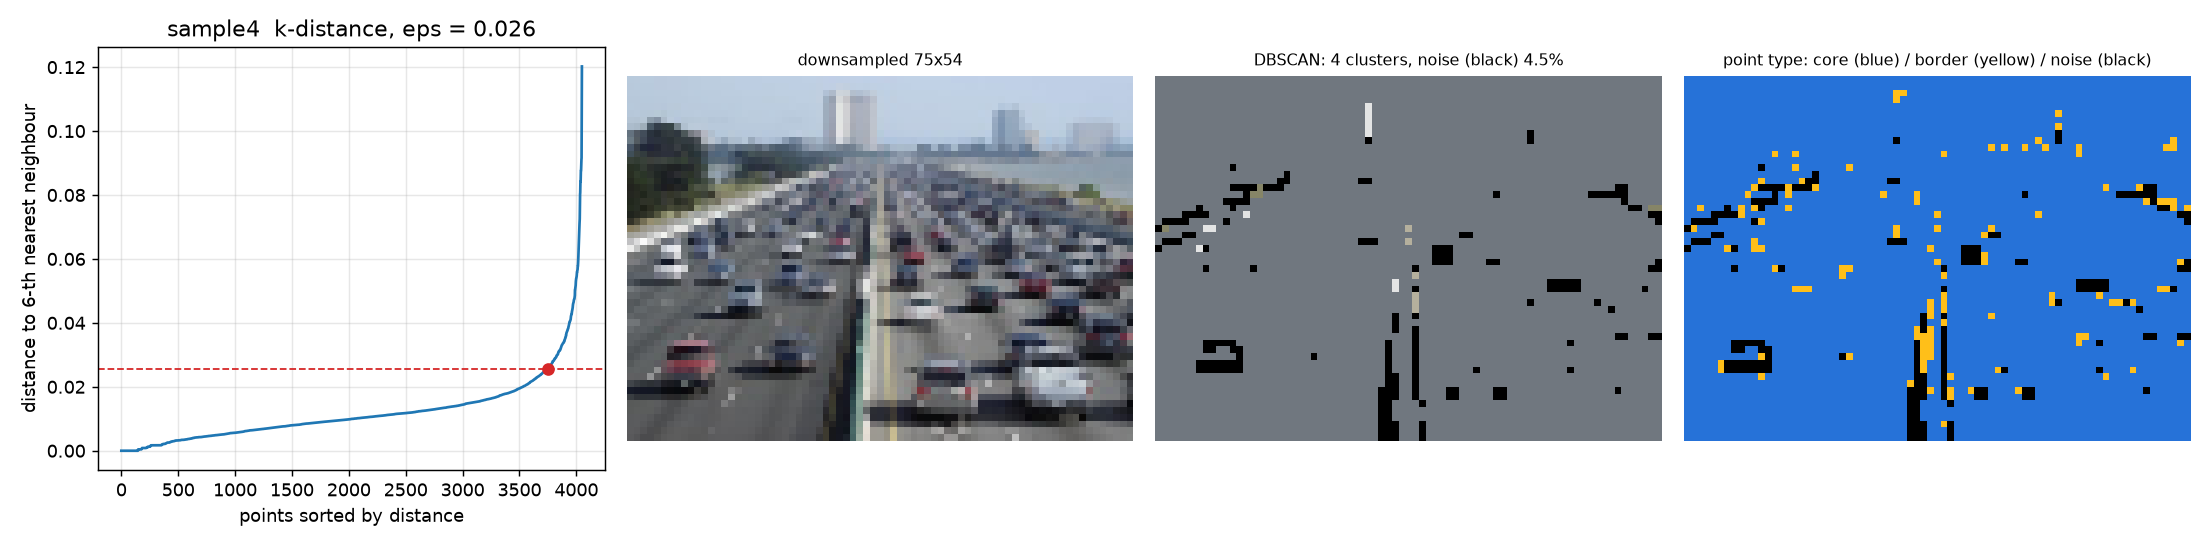
\includegraphics[width=\textwidth]{e_dbscan_sample4.png}\\[2pt]
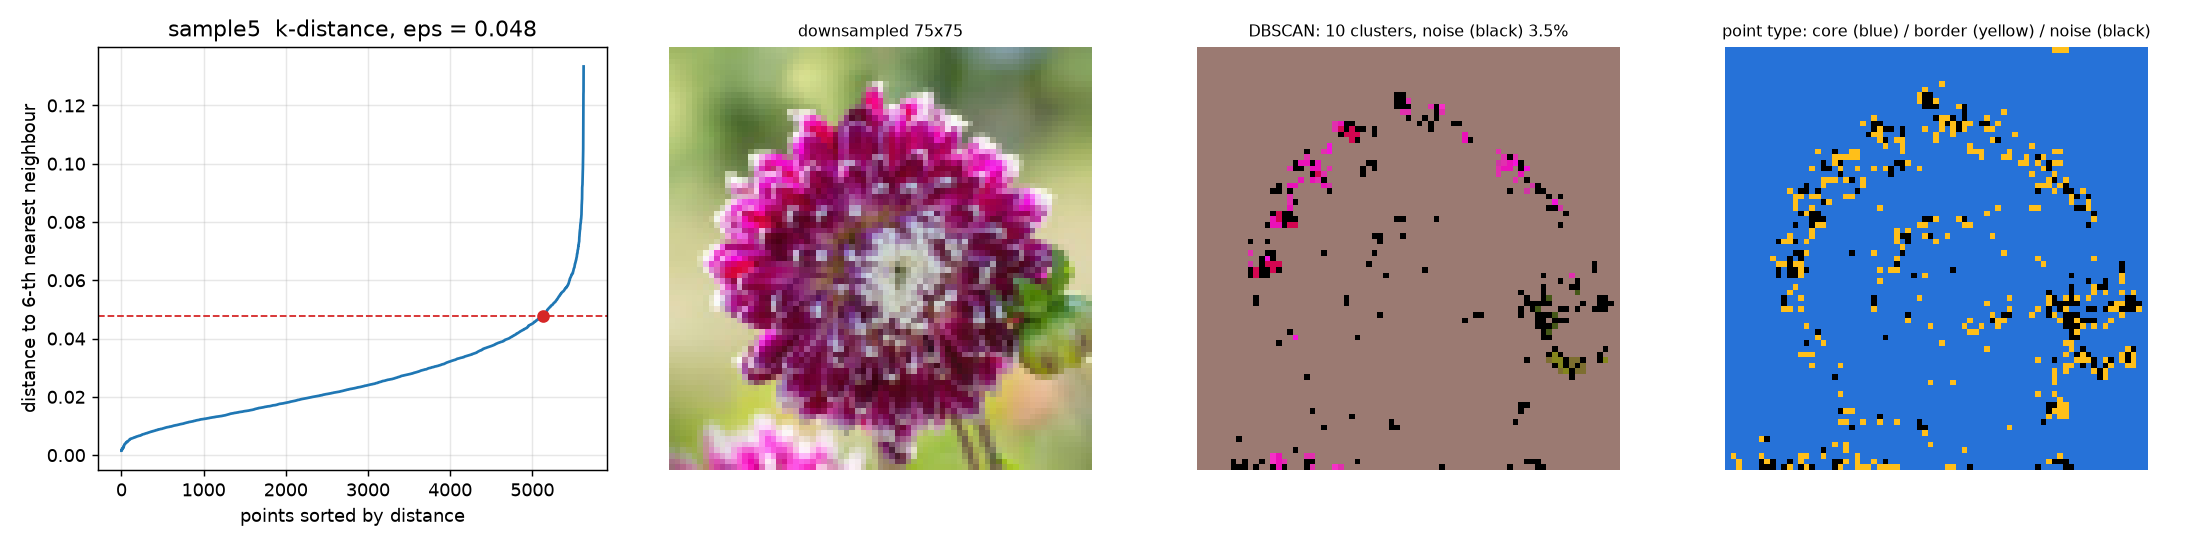
\includegraphics[width=\textwidth]{e_dbscan_sample5.png}
\caption{DBSCAN on \texttt{sample4} and \texttt{sample5}.}
\end{figure}

\subsection{K-Means vs.\ DBSCAN}

\textbf{(a) Shapes.} \emph{Rings:} 800 points on radii 1 and 2.5 with Gaussian radial noise ($\sigma=0.08$).
\emph{Blobs:} three Gaussian blobs ($\sigma=0.8$) plus 5\% uniform outliers. K-Means uses $K=2$ and $K=3$.
DBSCAN uses $\texttt{minPts}=5$ and $\varepsilon$ from the k-distance elbow. Quality is the adjusted Rand
index (ARI) against the true labels: 1 means perfect, 0 means no better than chance.

\begin{figure}[H]\centering
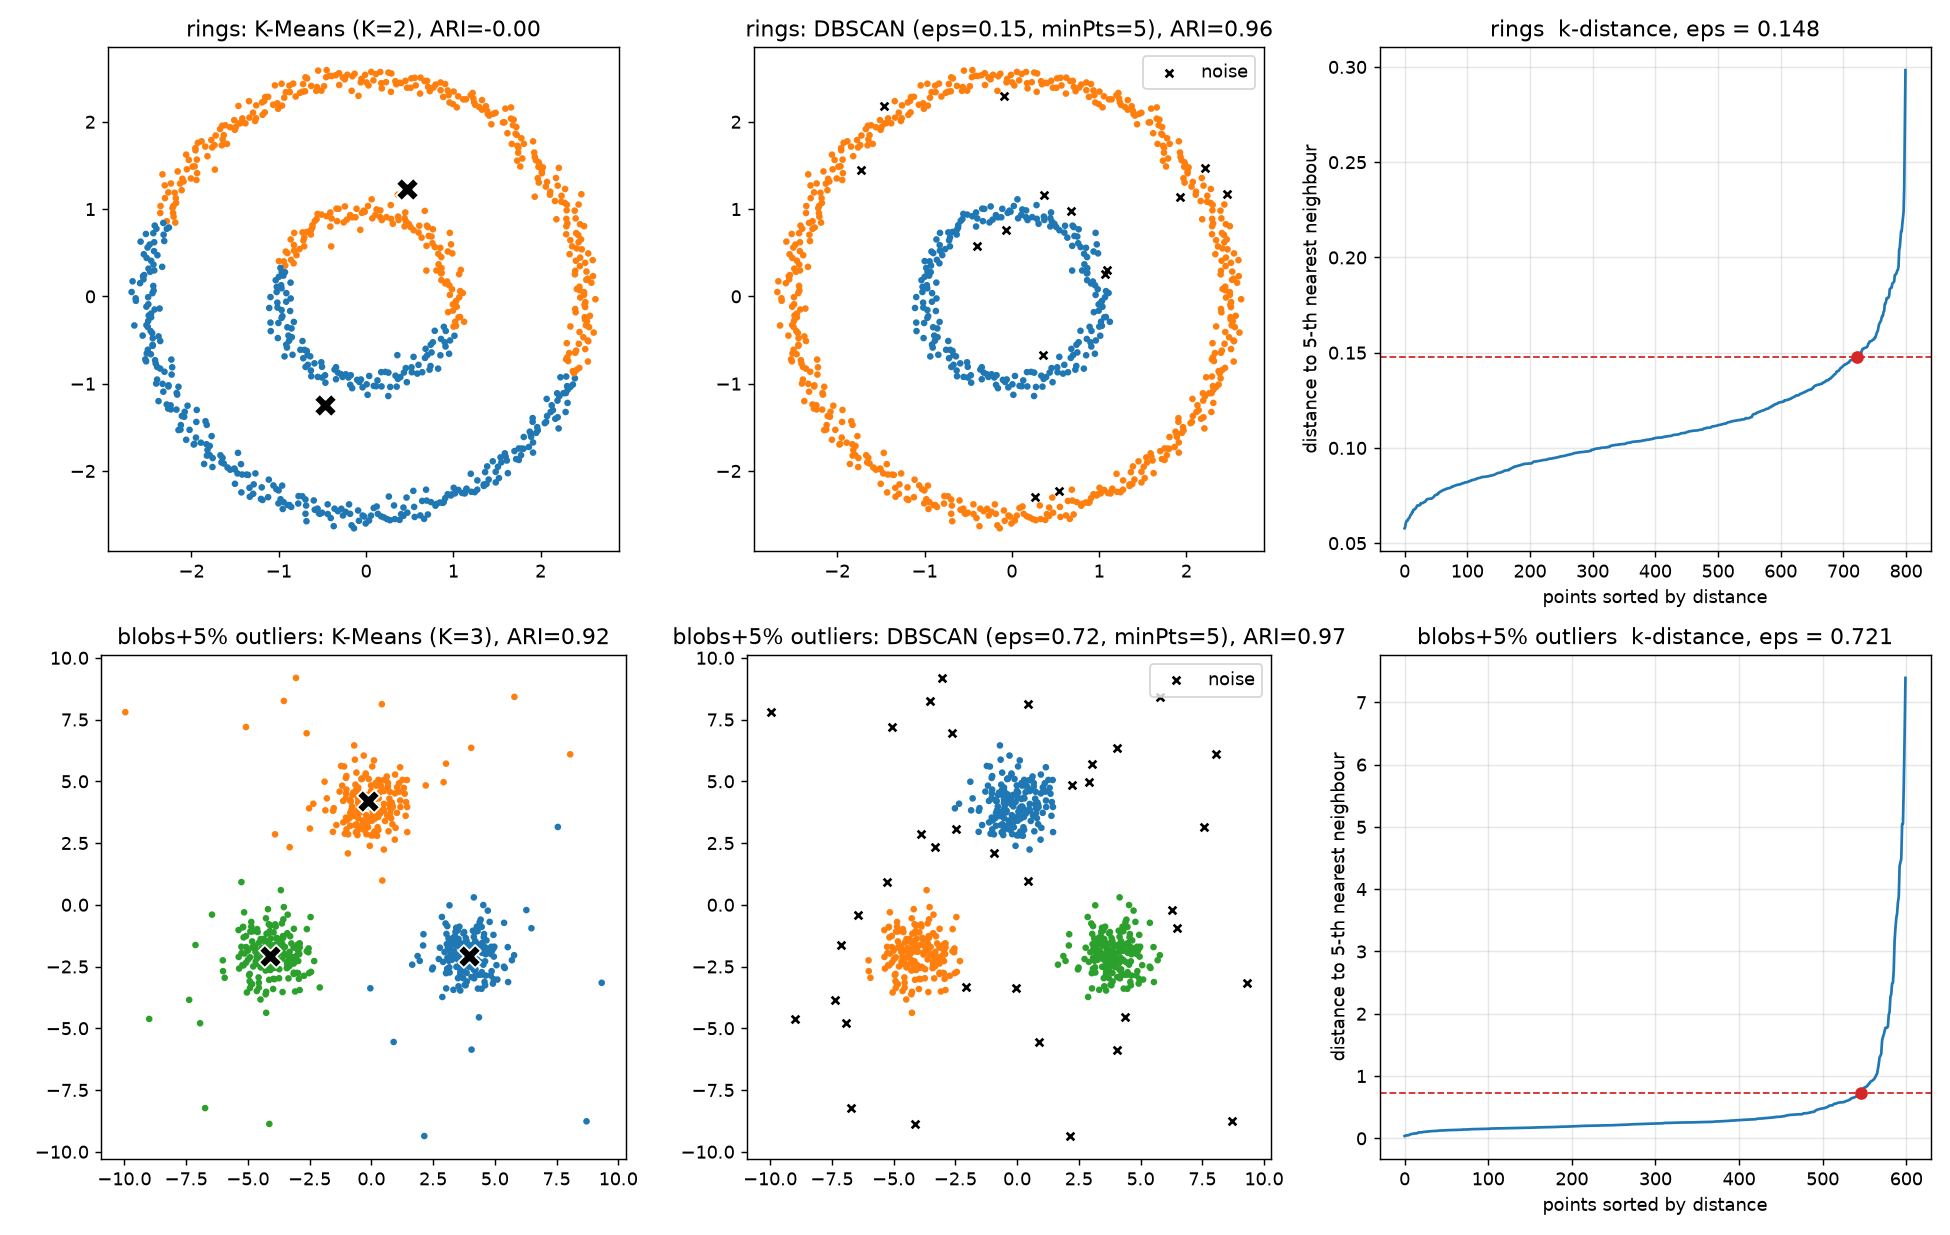
\includegraphics[width=\textwidth]{f_shapes.png}
\caption{K-Means (left), DBSCAN (middle, noise as black crosses) and the k-distance plot used to pick $\varepsilon$ (right).}
\end{figure}

\textbf{(b) Images.} \texttt{sample1} (natural) and \texttt{sample2} (flat shapes), downsampled as for DBSCAN.
We use K-Means with $K=16$ (our chosen $K$) and DBSCAN with $\varepsilon$ from the elbow, on RGB features and on
$(R,G,B,\lambda x,\lambda y)$ with $x,y\in[0,1]$ and $\lambda=0.5$.

\begin{figure}[H]\centering
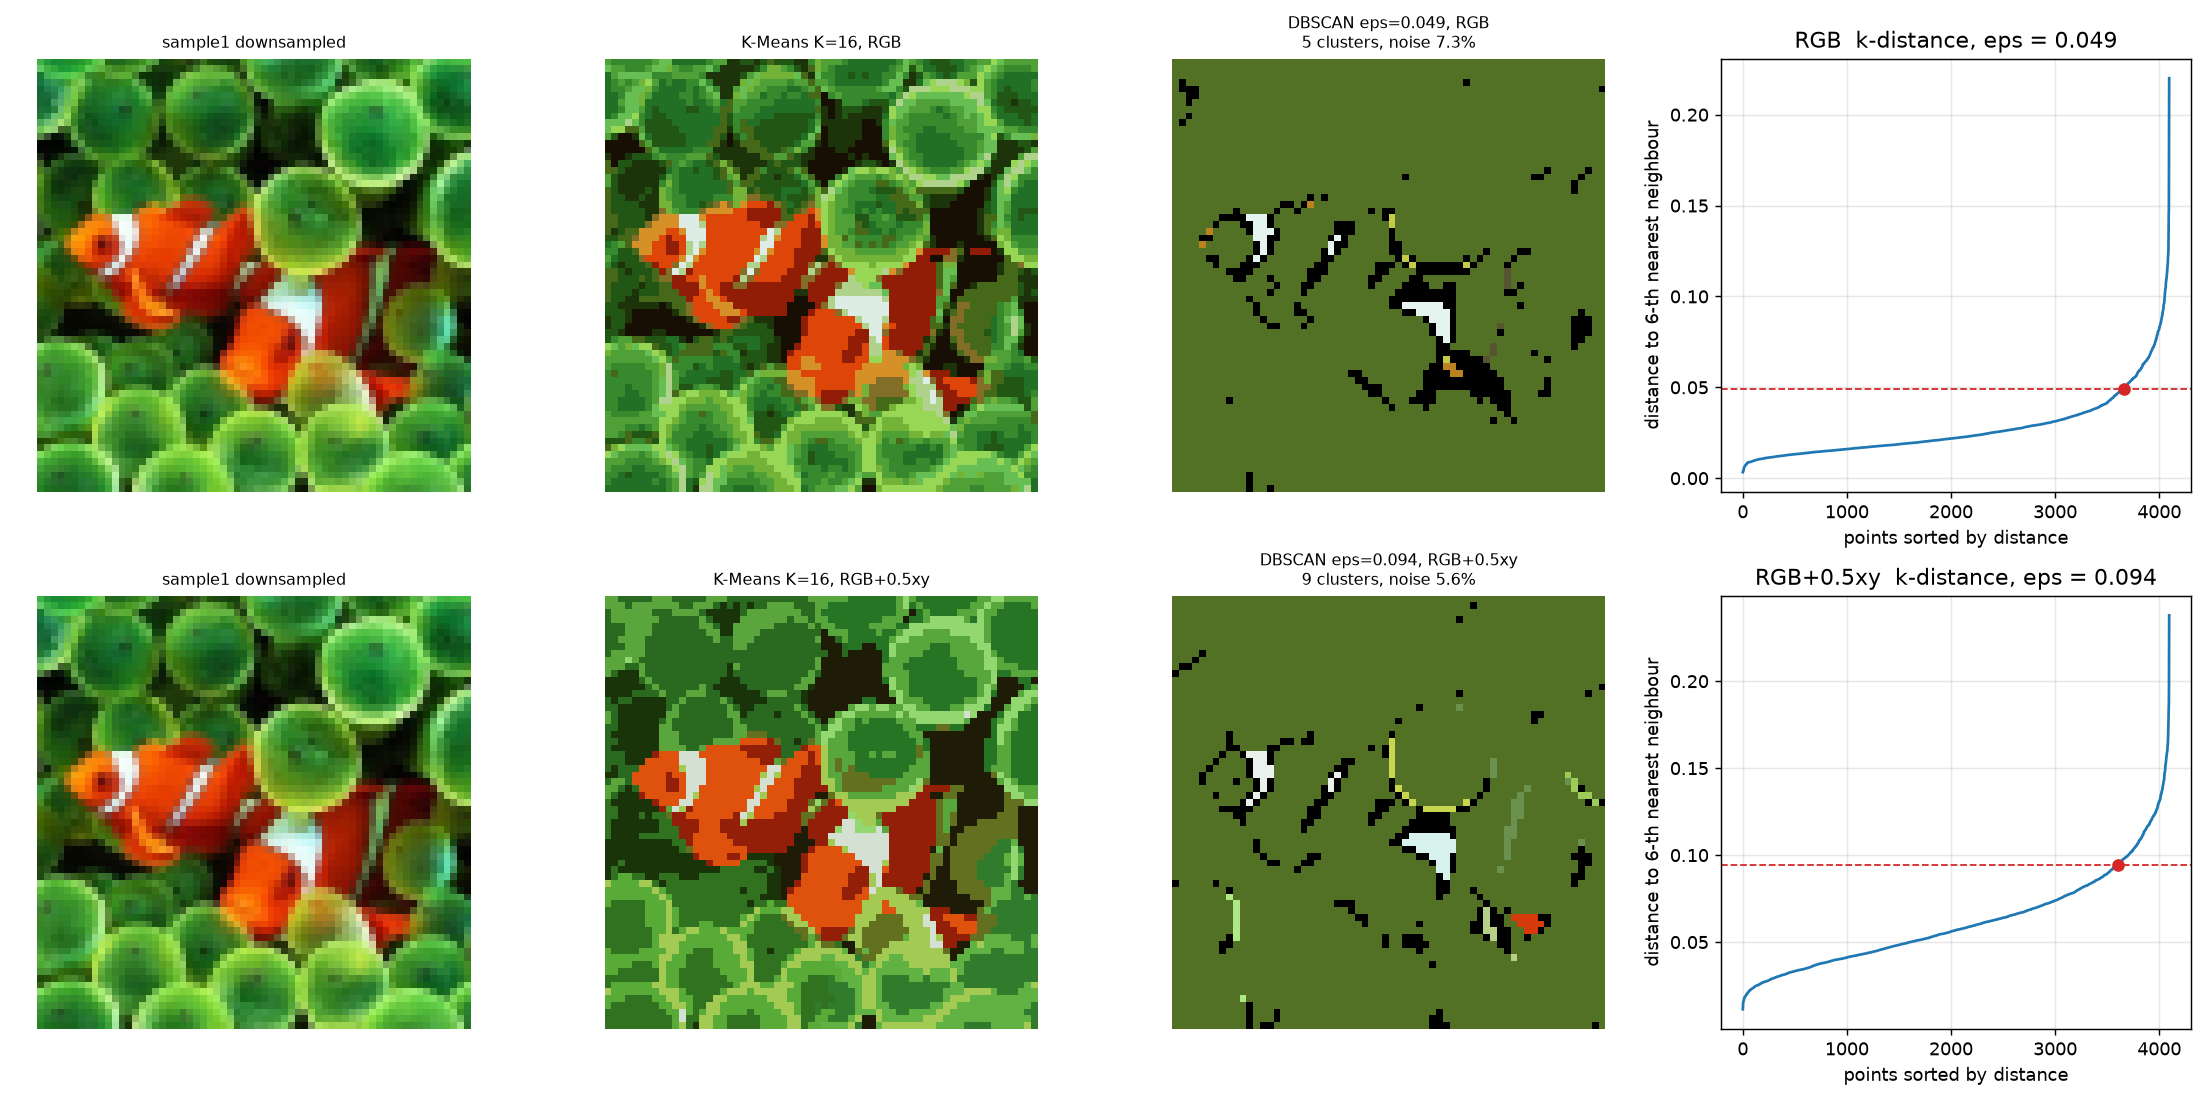
\includegraphics[width=\textwidth]{f_images_sample1.png}\\[2pt]
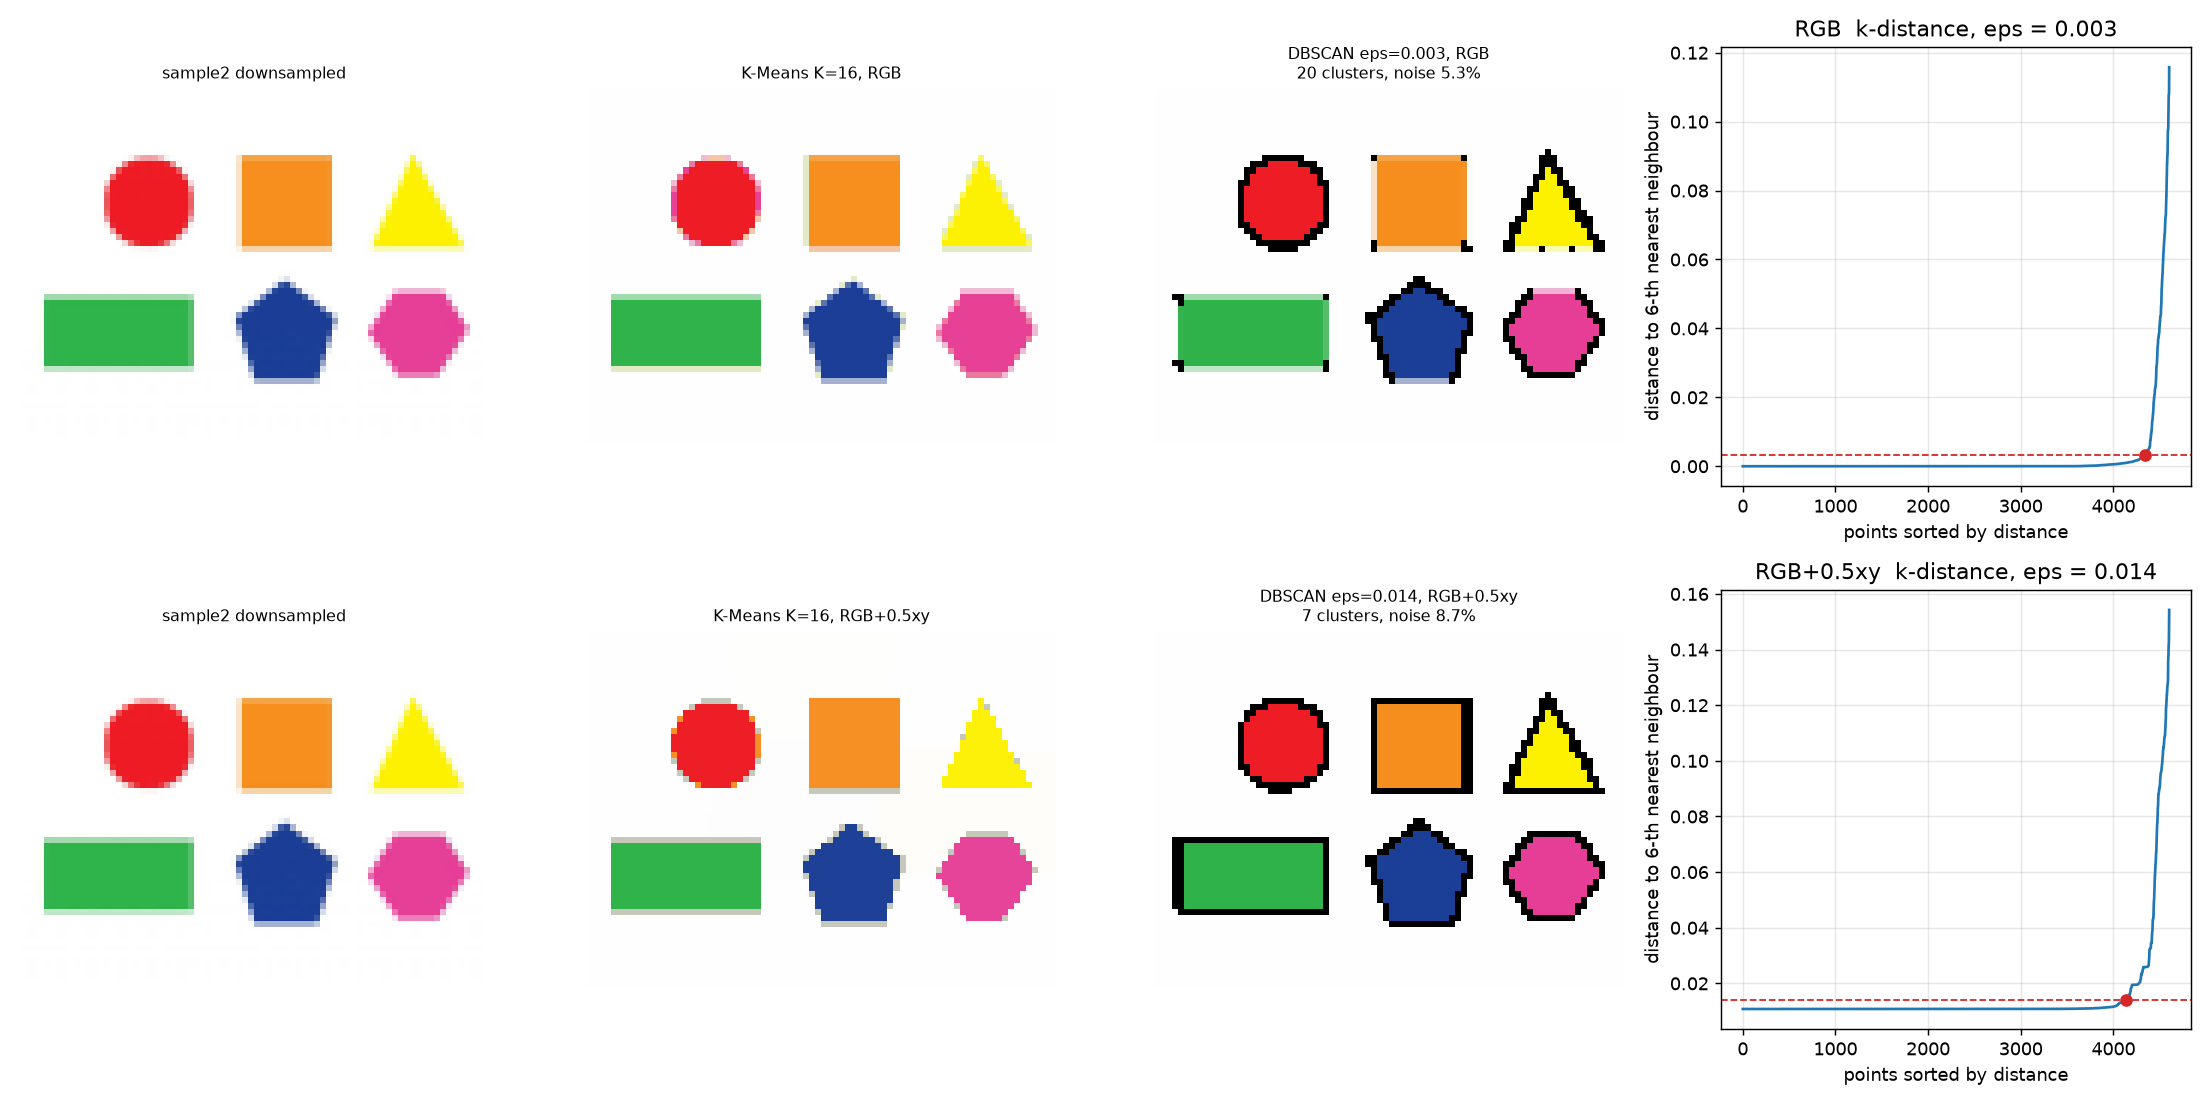
\includegraphics[width=\textwidth]{f_images_sample2.png}
\caption{Top two rows: \texttt{sample1}; bottom two rows: \texttt{sample2}. In each pair, the first row uses RGB
features and the second uses RGB$+0.5xy$.}
\end{figure}

\textbf{(c) Sensitivity} on the same two images (RGB features).
$\varepsilon$ is varied by $\pm30\%$ and $K$ by $\pm2$.

\begin{table}[H]\centering\small
\setlength{\tabcolsep}{4pt}
\resizebox{\textwidth}{!}{\begin{tabular}{llllrrrl}
\toprule
exp. & data & method & setting & clusters & noise \% & time (s) & quality / note\\
\midrule
\multirow{4}{*}{(a)} & rings & K-Means & $K=2$ & 2 & 0 & 0.002 & ARI $-0.00$: straight cut through both rings\\
 & rings & DBSCAN & $\varepsilon=0.148$ & 2 & 1.9 & 0.048 & ARI \textbf{0.96}: one cluster per ring\\
 & blobs+out. & K-Means & $K=3$ & 3 & 0 & 0.001 & ARI 0.92: outliers forced into blobs\\
 & blobs+out. & DBSCAN & $\varepsilon=0.721$ & 3 & 6.0 & 0.011 & ARI \textbf{0.97}: 93\% of outliers flagged\\
\midrule
\multirow{8}{*}{(b)} & sample1 & K-Means & RGB, $K=16$ & 16 & 0 & 0.031 & full 16-colour palette\\
 & sample1 & DBSCAN & RGB, $\varepsilon=0.049$ & 5 (1) & 7.3 & 0.22 & one giant cluster\\
 & sample1 & K-Means & RGB$+xy$, $K=16$ & 16 & 0 & 0.025 & colour + spatial patches\\
 & sample1 & DBSCAN & RGB$+xy$, $\varepsilon=0.094$ & 9 (1) & 5.6 & 0.25 & still one giant cluster\\
 & sample2 & K-Means & RGB, $K=16$ & 16 & 0 & 0.007 & 7 colours + 9 edge shades\\
 & sample2 & DBSCAN & RGB, $\varepsilon=0.0032$ & 20 (7) & 5.3 & 0.48 & 7 regions, edges = noise\\
 & sample2 & K-Means & RGB$+xy$, $K=16$ & 16 & 0 & 0.018 & background split into tiles\\
 & sample2 & DBSCAN & RGB$+xy$, $\varepsilon=0.014$ & 7 (7) & 8.7 & 0.27 & exactly background + 6 shapes\\
\midrule
\multirow{12}{*}{(c)} & sample1 & DBSCAN & $\varepsilon-30\%$ (0.034) & 12 (3) & 15.3 & 0.35 & \\
 & sample1 & DBSCAN & $\varepsilon$ (0.049) & 5 (1) & 7.3 & 0.26 & \\
 & sample1 & DBSCAN & $\varepsilon+30\%$ (0.064) & 10 (2) & 2.9 & 0.22 & \\
 & sample1 & K-Means & $K=14 / 16 / 18$ & 14 / 16 / 18 & 0 & 0.02--0.03 & SSE 41.7 / 37.9 / 32.0\\
 & sample2 & DBSCAN & $\varepsilon-30\%$ (0.0023) & 24 (7) & 5.8 & 0.44 & \\
 & sample2 & DBSCAN & $\varepsilon$ (0.0032) & 20 (7) & 5.3 & 0.56 & \\
 & sample2 & DBSCAN & $\varepsilon+30\%$ (0.0042) & 22 (7) & 4.8 & 0.46 & \\
 & sample2 & K-Means & $K=14 / 16 / 18$ & 14 / 16 / 18 & 0 & 0.005--0.007 & SSE 4.68 / 3.86 / 2.62\\
\bottomrule
\end{tabular}}
\caption{Summary of all three experiments. ``clusters'' gives the total, with the number of clusters holding at least
1\% of the points in brackets. Times for (b) and (c) are on the downsampled images ($\approx4$--5k points).}
\end{table}

\textbf{What the experiments show.}
\begin{itemize}
  \item \textbf{Shape.} K-Means can only make convex (Voronoi) regions, so it cuts the rings in half (ARI $\approx 0$).
        DBSCAN follows the density and separates both rings.
  \item \textbf{Outliers.} K-Means must assign every outlier to a blob, which pulls the centroids (by up to 0.16 units).
        DBSCAN flags 93\% of the true outliers as noise and scores a higher ARI (0.97 vs.\ 0.92).
  \item \textbf{Images.} K-Means gives exactly the requested palette and is the right tool for quantization. DBSCAN
        collapses natural images into one cluster, but gives a clean segmentation of the flat-colour \texttt{sample2}. With
        spatial features, it separates the six shapes perfectly (7 clusters), while K-Means wastes centroids on
        splitting the uniform background into spatial tiles.
  \item \textbf{Sensitivity.} K-Means responds smoothly to $K$: the cluster count equals $K$ and the SSE changes by
        about 10\% per step. DBSCAN on \texttt{sample1} is unstable. A 30\% smaller $\varepsilon$ doubles the noise
        (7.3\%$\to$15.3\%) and changes the cluster count from 5 to 12, and the number of large clusters is not even
        monotonic in $\varepsilon$ (3, 1, 2). On \texttt{sample2} the 7 regions survive the whole $\pm30\%$ range,
        because they are separated by large gaps in colour space.
  \item \textbf{Running time.} On the same $\approx$4k points, K-Means takes 5--30\,ms and DBSCAN 200--600\,ms.
        DBSCAN needs all pairwise distances, $O(n^2)$, so the full $788{,}480$-pixel image would need about
        $6\times10^{11}$ distances. K-Means costs $O(nK)$ per iteration and quantizes the full image in about 1\,s.
\end{itemize}

\textbf{Conclusion.} We would choose K-Means when the number of groups is known or set by the task, as in
quantization, where $K$ fixes the bit budget. It is also the choice when clusters are roughly round and the data
are large, since it scales linearly with the number of points and behaves predictably as $K$ changes. We would
choose DBSCAN when clusters have arbitrary shapes (rings, elongated regions) or the data contain outliers that
should be flagged rather than absorbed, and it has the added advantage that it finds the number of clusters by
itself. DBSCAN's weaknesses are its sensitivity to $\varepsilon$ (a $\pm30\%$ change can double the noise or merge
regions), its $O(n^2)$ cost, which forced us to downsample to $80\times80$, and its failure on data with no
density gaps, such as the continuous colour distributions of natural photographs. For colour quantization,
K-Means is the clear choice. DBSCAN is better suited to segmenting flat-colour graphics or detecting unusual
colours.

%======================================================================
\section{Q2 -- Warehouse robot with Value Iteration}
%======================================================================

\textbf{Model.} Every non-shelf cell is a state, and \texttt{G} and \texttt{X} are terminal with fixed values $+100$ and $-100$.
We use the same update as Part A2:
\[
V_{k+1}(s)=\max_a\Big[r+\gamma\sum_{s'}P(s'\mid s,a)\,V_k(s')\Big],
\]
with a synchronous update (all states use $V_k$). Moving into a shelf or off the grid leaves the robot in place.
Transitions are stored as an array \texttt{nxt[a, s, j]} (the state reached by outcome $j$: intended, slip left, slip right)
together with the outcome probabilities $(1,0,0)$ or $(0.8,0.1,0.1)$. One backup of all states is then a single
vectorised line, \texttt{Q = r + gamma * V[nxt] @ probs}. Unless stated otherwise, $\gamma=0.9$, $r=-1$ and
$\theta=10^{-4}$. Ties in the greedy policy go to the first action in the order U, D, L, R.

\textbf{Map} (\texttt{warehouse-1.txt}). Start \texttt{S} is at (7,0) and \texttt{G} at (7,9). Row 7 is a 9-step corridor running
directly under the three spill cells (6,3)--(6,5). The safe alternative goes up column 0, along row 4 and down
column 9, which takes 15 steps.
\begin{center}\small
\begin{tabular}{c}
\texttt{..........}\\[-2pt]
\texttt{.\#\#.\#\#.\#\#.}\\[-2pt]
\texttt{.\#\#.\#\#.\#\#.}\\[-2pt]
\texttt{.\#\#.\#\#.\#\#.}\\[-2pt]
\texttt{..........}\\[-2pt]
\texttt{.\#\#\#\#\#\#\#\#.}\\[-2pt]
\texttt{.\#\#XXX\#\#\#.}\\[-2pt]
\texttt{S........G}\\[-2pt]
\texttt{\#\#\#\#\#\#\#\#\#\#}\\[-2pt]
\texttt{\#\#\#\#\#\#\#\#\#\#}
\end{tabular}
\end{center}

\subsection{Deterministic Value Iteration}

\textbf{Value Iteration converges in 17 iterations} (largest change $<10^{-4}$), with $V^*(S)=32.62$. The greedy policy
takes the shortest route, straight along the corridor (9 steps). Values rise smoothly towards \texttt{G}:
each step away multiplies the remaining value by $\gamma$ and costs 1.

\begin{figure}[H]\centering
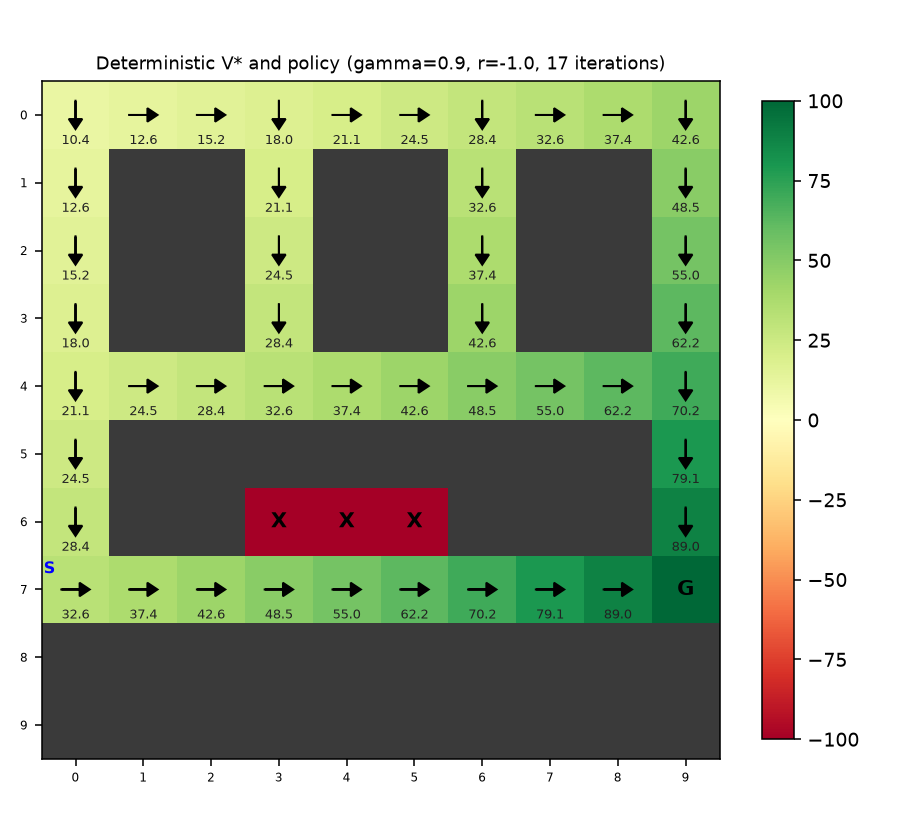
\includegraphics[width=0.58\textwidth]{a_deterministic.png}
\caption{Deterministic world: heatmap of $V^*$ with greedy policy arrows (shelves in grey).}
\end{figure}

\subsection{Stochastic Value Iteration}

With slip probabilities $0.8/0.1/0.1$, \textbf{Value Iteration converges in 38 iterations}, and $V^*(S)$ drops to $4.44$.
The policy changes in 8 cells (magenta in the figure):

\begin{table}[H]\centering\small
\resizebox{\textwidth}{!}{\begin{tabular}{lccrrl}
\toprule
cell & deterministic & stochastic & $V^*$ det. & $V^*$ stoch. & reason\\
\midrule
(7,0) = S & R & \textbf{U} & 32.62 & 4.44 & avoid the spill corridor, take the long safe route\\
(7,1) & R & \textbf{L} & 37.35 & 2.68 & go \emph{back} to S and up rather than pass the spills\\
(6,0), (5,0) & D & \textbf{U} & 28.35, 24.52 & 6.67, 8.98 & climb towards row 4 instead of descending\\
(4,0) & D (tie) & \textbf{R} & 21.07 & 11.62 & safe row 4 instead of the corridor\\
(0,0), (0,3), (0,6) & D (tie) & \textbf{R} & 10.4--28.4 & 3.8--19.6 & deterministic tie broken by the slip dynamics\\
\bottomrule
\end{tabular}}
\caption{Cells where the stochastic policy differs from the deterministic one.}
\end{table}

\textbf{Why.} In the deterministic world, the corridor is simply the shortest path. In the stochastic world, every
horizontal move in cells (7,3), (7,4) and (7,5) has a 10\% chance of slipping \emph{up} into a spill ($-100$).
Crossing those three cells succeeds only about $0.9^3\approx73\%$ of the time, and slips down into the shelf
cost extra steps on top of that. The safe route is 6 steps longer, but no spill sits next to it, so for
$\gamma=0.9$, $r=-1$ the optimal robot turns \emph{up} at \texttt{S}. The most striking cell is (7,1): there the
optimal action is to step \emph{back} (L) to \texttt{S} and take the long way round. In (4,0) and (0,0), (0,3), (0,6),
the deterministic Q-values for D and R are exactly equal (for example (0,0): $Q_D=Q_R=10.383$), and the tie-break
picks D. Under slipping, the routes are no longer equivalent, because the D routes lead towards the risky
corridor or into aisles where slips are wasted against shelves, so R becomes strictly better. Every value is
lower in the stochastic world, both because of the spill risk and because slips into walls waste steps
(each costing $r$ and a factor $\gamma$).

\begin{figure}[H]\centering
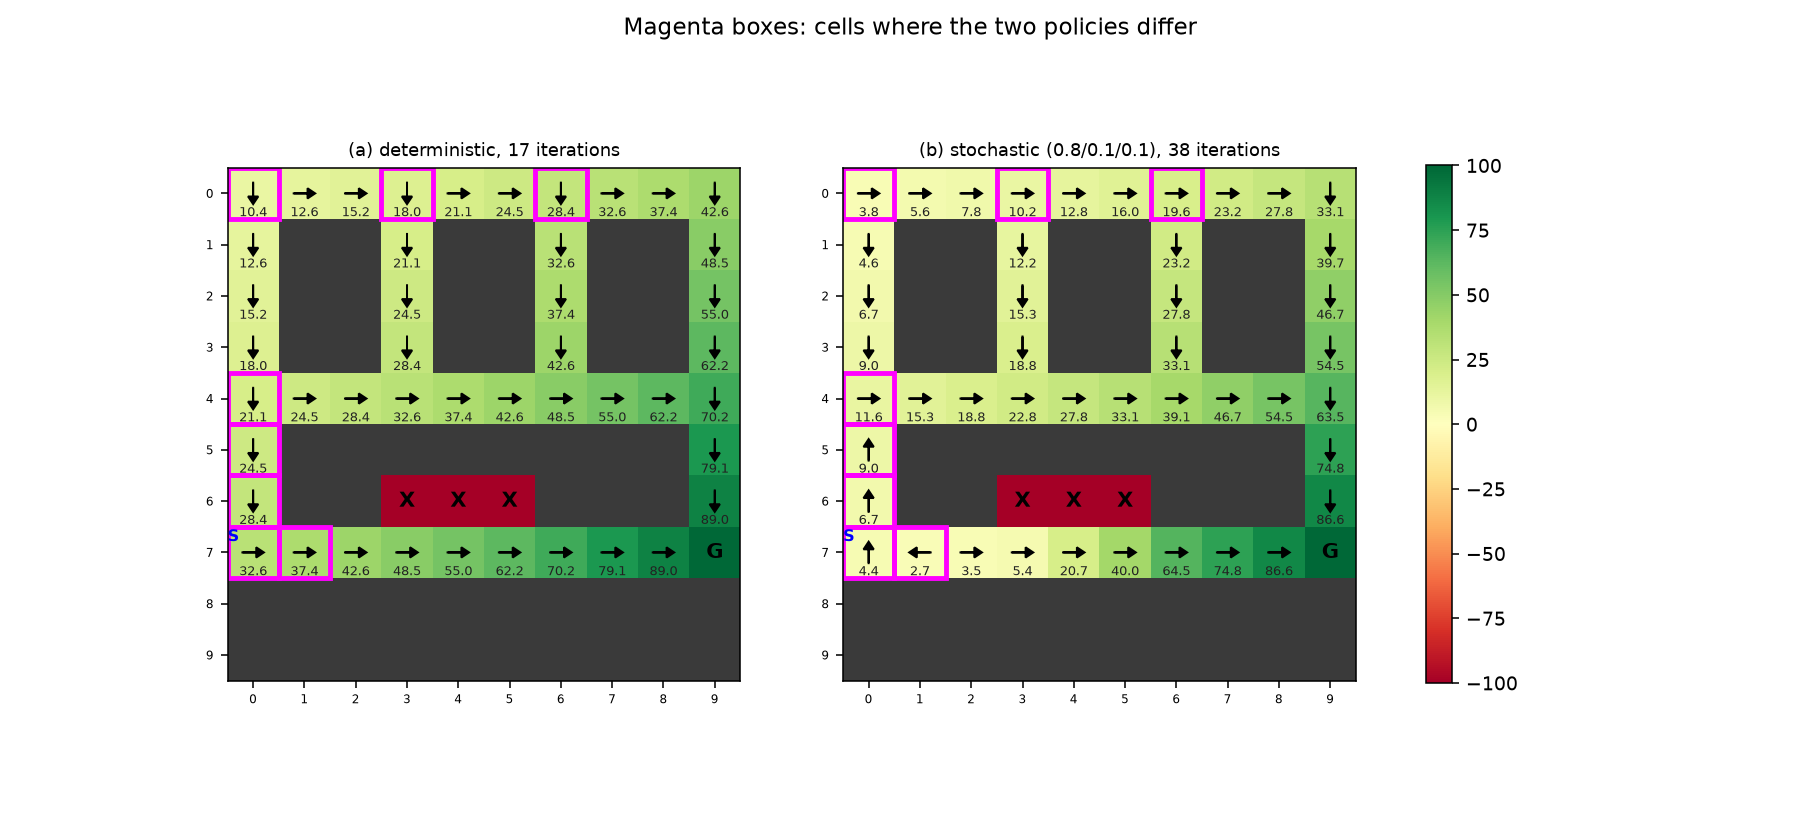
\includegraphics[width=\textwidth]{b_stochastic_vs_deterministic.png}
\caption{Deterministic (left) vs.\ stochastic (right) $V^*$ and policy. Magenta boxes mark the 8 cells whose action changed.}
\end{figure}

\subsection{Evaluating policies by simulation}

\texttt{simulate(policy, episodes=1000)} runs 1000 episodes of the \emph{stochastic} world from \texttt{S} (vectorised over episodes,
seed 0, capped at 500 steps). The return of an episode is the undiscounted sum $r\cdot\text{steps}+(\pm100)$. As a cross-check,
the last column gives the exact discounted value $V^\pi(S)$ of each policy in the stochastic world, from solving the linear
Bellman equations.

\begin{table}[H]\centering\small
\begin{tabular}{lrrrrrr}
\toprule
policy (run in the stochastic world) & avg return & avg steps & success \% & spill \% & steps (successes) & $V^\pi(S)$\\
\midrule
deterministic-world policy & 25.8 & 9.4 & 67.6 & 32.4 & 11.0 & 0.27\\
stochastic-world policy & \textbf{80.3} & 19.7 & \textbf{100.0} & \textbf{0.0} & 19.7 & \textbf{4.44}\\
\bottomrule
\end{tabular}
\caption{Both policies evaluated in the stochastic world (1000 episodes, $r=-1$).}
\end{table}

The deterministic-world policy is faster when it works, but about a third of its runs end in a spill. That is even
worse than the $0.9^3$ estimate, because a slip down into the shelf keeps the robot in a dangerous cell for another
attempt. The stochastic-world policy never spills and has a much higher average return (80.3 vs.\ 25.8), at the cost
of about 10 extra steps. The ranking matches the exact values $V^\pi(S)$ ($4.44>0.27$).

\subsection{Discount and living reward}

Stochastic Value Iteration was run for all 12 combinations, and each policy was simulated for 1000 episodes.

\begin{table}[H]\centering\small
\begin{tabular}{rrrrrrrrr}
\toprule
$\gamma$ & $r$ & iterations & success \% & spill \% & timeout \% & avg steps & avg return & $V^*(S)$\\
\midrule
0.5 & $-5$ & 17 & 100 & 0 & 0 & 64.1 & $-220.3$ & $-10.00$\\
0.5 & $-1$ & 18 & 100 & 0 & 0 & 64.1 & 35.9 & $-2.00$\\
0.5 & 0 & 18 & 100 & 0 & 0 & 64.1 & 100.0 & 0.00\\
0.5 & $+1$ & 18 & 100 & 0 & 0 & 64.1 & 164.1 & 2.00\\
\midrule
0.9 & $-5$ & 37 & \textbf{72.1} & \textbf{27.9} & 0 & \textbf{10.4} & $-7.9$ & $-24.36$\\
0.9 & $-1$ & 38 & 100 & 0 & 0 & 19.7 & 80.3 & 4.44\\
0.9 & 0 & 49 & 100 & 0 & 0 & 19.7 & 100.0 & 13.13\\
0.9 & $+1$ & 51 & 100 & 0 & 0 & 19.7 & 119.7 & 21.82\\
\midrule
0.99 & $-5$ & 42 & 96.0 & 4.0 & 0 & 18.3 & 0.7 & $-6.40$\\
0.99 & $-1$ & 104 & 100 & 0 & 0 & 19.7 & 80.3 & 64.17\\
0.99 & 0 & 162 & 100 & 0 & 0 & 19.7 & 100.0 & 82.08\\
0.99 & $+1$ & 168 & \textbf{0} & 0 & \textbf{100} & 500 & 500 & 100.00\\
\bottomrule
\end{tabular}
\caption{Stochastic Value Iteration for every $(\gamma,r)$ combination. ``Timeout'' means the 500-step cap was reached.}
\end{table}

\begin{figure}[H]\centering
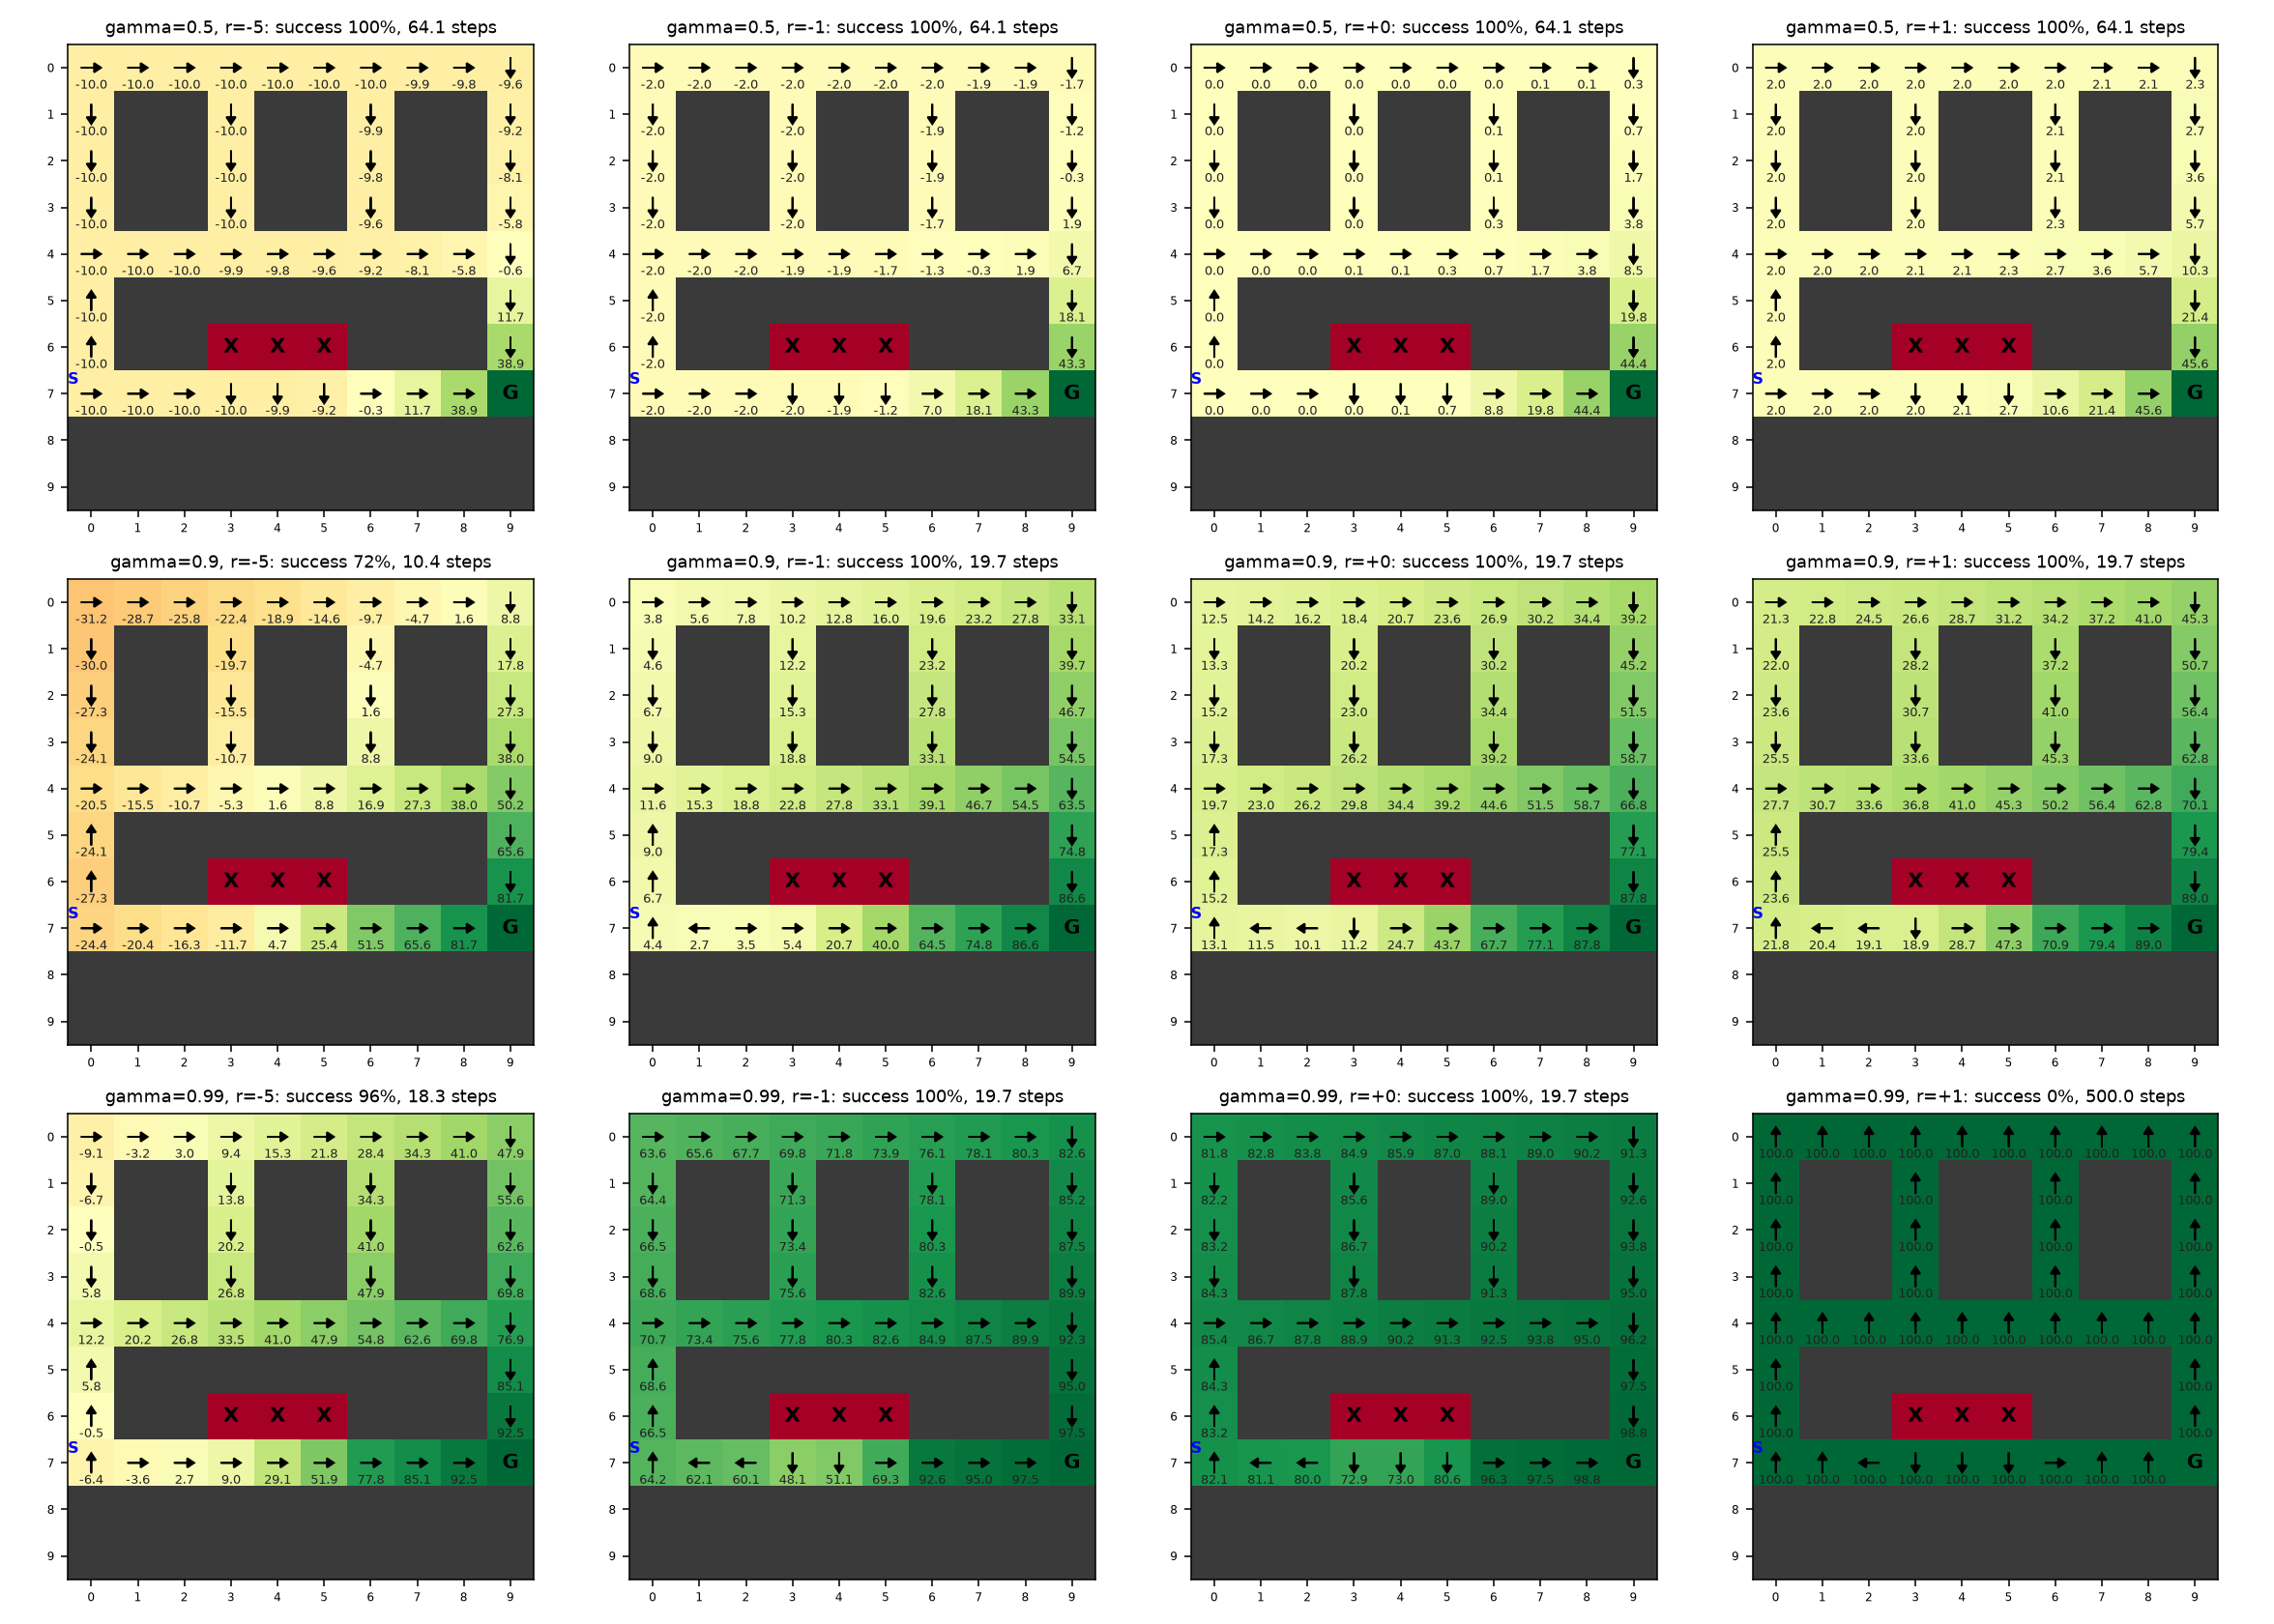
\includegraphics[width=\textwidth]{d_sweep_policies.png}
\caption{Policy maps for all 12 settings (rows: $\gamma=0.5,0.9,0.99$; columns: $r=-5,-1,0,+1$).}
\end{figure}

\begin{itemize}
  \item \textbf{Takes risks} ($\gamma=0.9$, $r=-5$). Each step costs 5, so the 6 extra steps of the safe route cost more than
        the expected spill penalty. The robot goes straight down the corridor: 72\% success, 28\% spills, only 10.4 steps.
        With $\gamma=0.99$, $r=-5$ the robot starts on the safe route (U at \texttt{S}). But if it slips right into (7,1),
        it commits to the corridor (R), because going back now costs more. This gives 96\% success and 4\% spills, a mixed strategy.
  \item \textbf{Plays safe} ($r\in\{-1,0\}$ for $\gamma=0.9$ and $0.99$, and $r=+1$ with $\gamma=0.9$). The robot always takes the
        spill-free route: 100\% success in 19.7 steps. When steps are cheap or free, a few extra moves cost almost nothing
        compared with a $-100$ spill.
  \item \textbf{Short-sighted} ($\gamma=0.5$, all $r$). Seen from \texttt{S}, the reward is $100\cdot0.5^{d}$ for a goal $d$ steps away, which is
        negligible ($0.5^{9}\cdot100\approx0.2$). Values far from \texttt{G} sit at $r/(1-\gamma)$, as if the goal did not exist.
        The robot drifts into the corridor and, beneath the spills, chooses \textbf{D} (into the shelf). The intended move leaves it
        in place, and only the 10\% sideways slips move it, so it shuffles along with zero spill risk. It always arrives, but takes
        64 steps on average. The policy is the same for all four values of $r$.
  \item \textbf{Never reaches the station} ($\gamma=0.99$, $r=+1$). Living forever is worth $\sum_t\gamma^t r=r/(1-\gamma)=100$, and reaching
        \texttt{G} after any $t$ steps is worth $(1-\gamma^t)/(1-\gamma)+100\gamma^t=100$ as well, so every safe action ties at
        $V=100$. Entering a spill is strictly worse, so the robot stays out of trouble and simply wanders (here it pushes U
        against walls): 0\% success, and every episode hits the 500-step cap. The ``return'' of 500 only reflects the cap.
        With $\gamma=0.9$, staying forever is worth only 10, while reaching \texttt{G} is worth far more, so the robot still goes to \texttt{G}.
  \item \textbf{Iterations grow with $\gamma$} (17--18 for $\gamma=0.5$, 37--51 for $0.9$, 42--168 for $0.99$). The Bellman update is a $\gamma$-contraction, so the error
        shrinks roughly like $\gamma^k$, and larger $\gamma$ also propagates information from \texttt{G} further.
\end{itemize}

\subsection{Bonus: Policy Iteration vs.\ Value Iteration}

Policy Iteration starts from ``always U''. It evaluates the policy exactly by solving the linear system
$(I-\gamma P^\pi_{NN})V_N=r+\gamma P^\pi_{NT}V_T$, then improves it greedily, changing an action only on a strict improvement
($>10^{-9}$). It stops when no state changes. The comparison uses a random, reachable $20\times20$ map
(\texttt{random\_map}, seed 3, 22\% shelves, 12 spills, \texttt{S} at bottom-left, \texttt{G} at top-right) in the stochastic
world with $r=-1$. Times are the median of 5 runs.

\begin{table}[H]\centering\small
\begin{tabular}{rlrrl}
\toprule
$\gamma$ & method & iterations & time (ms) & agreement with VI\\
\midrule
0.9 & Value Iteration & 89 & 1.7 & --\\
0.9 & Policy Iteration & \textbf{9} & 65.8 & same action in 303/303 states, $\max|V_{PI}-V_{VI}|=8.5\times10^{-4}$\\
0.99 & Value Iteration & 918 & 16.1 & --\\
0.99 & Policy Iteration & \textbf{9} & 65.0 & same action in 302/303 states, $\max|V_{PI}-V_{VI}|=9.8\times10^{-3}$\\
\bottomrule
\end{tabular}
\caption{Policy Iteration vs.\ Value Iteration on the random $20\times20$ map.}
\end{table}

Policy Iteration needs \textbf{10--100$\times$ fewer iterations}, and its count does not depend on $\gamma$, whereas Value Iteration's
grows roughly like $1/(1-\gamma)$. Each PI iteration, however, solves a dense $303\times303$ linear system ($O(n^3)$), while each
VI sweep is one cheap vectorised backup ($O(4\cdot3\cdot n)$). So on this small map, VI is faster in wall-clock time
($4$--$40\times$), and the gap shrinks as $\gamma\to1$. Both methods reach the same policy. The single differing state at
$\gamma=0.99$ is a near-tie within VI's $\theta$ tolerance.

\begin{figure}[H]\centering
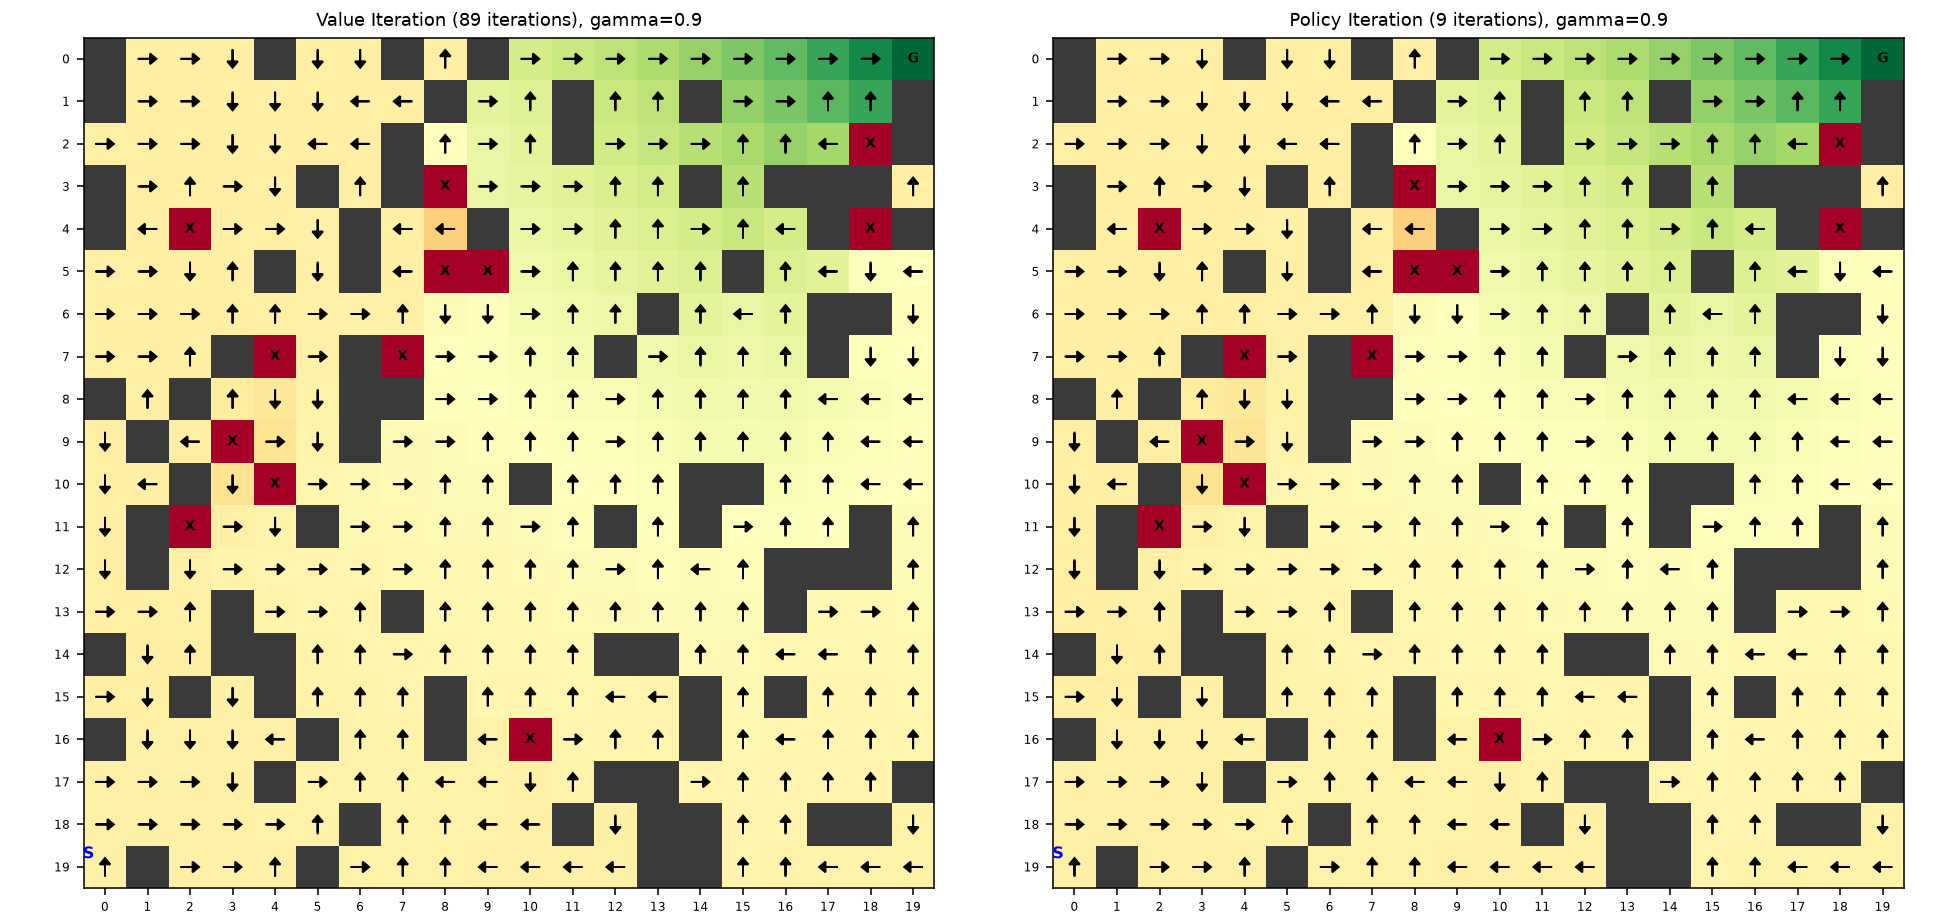
\includegraphics[width=\textwidth]{bonus_pi_vs_vi.png}
\caption{Random $20\times20$ map, $\gamma=0.9$: Value Iteration (left) and Policy Iteration (right) give the same policy.}
\end{figure}

\end{document}
